\chapter{関係データベースの設計 -- 実体関連モデル}\label{chap:er-model}

\ref{chap:anomaly}章では，データの挿入，削除，更新時に発生するデータベースの不都合である異状について説明しました．
データベースの異状を含め，データベースが常に正しく矛盾がない状態に保つためには，\ref{chap:relational-data-model}章で説明した関係データモデルの制約やテーブルの構造を適切に設計することが重要になってきます．

ところが，データベースを正しく設計することは想像以上に難しいことです．
これまでの章で説明に用いてきたテーブルは高々2，3個でした．
しかし，データ管理の現場では関係データベース内のテーブルの数が数十，数百になることはめずらしくありません．
また，データベース設計においては唯一の正解があるわけではなく，現実世界の複雑なルールやデータが用いられる文脈を紐解き，それをデータベース管理システムが扱える形に落とし込む必要があります．
そのため，どれほど経験があるデータエンジニアであっても，いきなり完全無欠でメンテナンスもしやすい関係データベースを設計することは難しいです．
データが正しく保たれ，冗長なデータも発生せず，かつ一貫性制約の保持が容易である関係データベースを設計するには，対象とする事象やその中に存在するルールに対する理解を深めた上で，体系的にデータモデルを構築する必要があります．

そこで本章および次章では，関係データベースの設計手法である\strong{実体関連モデルを変換する方法}および\strong{正規化}について解説します．


\section{データモデリングの流れ}
\ref{chap:concept-of-database}章で説明したように，データモデリングとは対象とする課題に応じて扱うべき情報を取捨選択し，データの構造，制約条件，操作方法を設計する行為です．
図\ref{fig:data_modeling_process}が示すように，一般にデータモデリングは概念モデリング，論理モデリングの順で行われます．
\begin{figure}[tb]
    \centering
    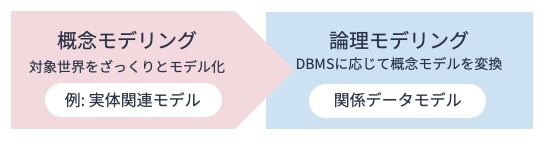
\includegraphics[width=0.8\textwidth]{figure/er-model/data-modeling-process.jpg}
    \caption{データモデリングの流れ}
    \label{fig:data_modeling_process}
\end{figure}

\strong{概念モデリング}は，最終的にどのようなデータベース技術を利用するかに関係なく，対象とする課題（例：ビジネスの業務要件）の全体像を把握した上で，扱おうとするデータ対象がどのようなものであるか（どのような意味を持つか）を記述する手続きです．
概念モデリングにおいては，本章で説明する実体関連モデルが用いられることが多いです．

\strong{論理モデリング}の過程では，概念モデリングで設計された概念モデルをデータベース管理システムが扱えるよう変換します．
例えば，データベース管理システムが関係データベース管理システムであれば，あらかじめ設計された概念モデルを関係データモデルに変換することになります．


本書では関係データベースの設計手法として，実体関連モデルに基づく方法と関数従属性にもとづく正規化の2種類の方法を学びます．
これらは二者択一ではなく，両方を組み合わせて用いることが実務におけるベストプラクティスです．
詳細は本章，次章で説明しますが，それぞれの利用シーンは以下の通りです：
\begin{description}
    \item[実体関連モデルに基づく方法]：何もない状況から対象課題の要件を整理し，データの構造や関連を俯瞰的に設計したい場合
    \item[データ従属性にもとづく正規化]：ある程度具体的なデータ項目（テーブルの属性）が出揃っている状況で，データの重複や異状が発生しないテーブル構造を導出したい場合
\end{description}

以降本章では，代表的な概念モデルである実体関連モデルを解説した後，実体関連モデルを関係データモデルに変換する方法について述べます．


\begin{notebox}{データモデリングは難しい!?}
本章および次章では「データベースの設計方法」を学びますが，学ばなければならない知識はそれほど多くありません．
例えば，本章で学ぶ実体関連モデルでは，主要概念は「実体」と「関連」の2種類しかありません．
内容も一見すると，大したことがないように見えます．
ところが，実際にデータベース設計ができるようになるには時間がかかります．
例えば，実体関連モデルの概念を学んだ初心者がいざ実体関連モデルを作ろうとすると，何をどうすればよいのか困るでしょうし，モデルを作ったもののそれが正しいものか不安になるでしょう．
設計は知識よりも経験（考え方の体得）がものを言うからです．
データモデリングのような抽象的な思考を体得するには，とにかく「やってみては間違えるを繰り返す」しかありません．
\end{notebox}



\section{実体関連モデルとは}
\strong{実体関連モデル（entity-relationship model; ERモデル）} は，Peter Chenにより提唱された概念モデリング用のデータモデルです\cite{Chen1976}．
実体関連モデルでは，実世界のデータのすべてを「実体」と「関連」の2種類で分類・記述します．
実体関連モデルを図として表現したものを\strong{実体関連図（entity-relationship diagram; ER図）} と呼びます．

実体関連モデルおよび実体関連図には様々な記法\footnote{本書で説明するPeter Chen記法以外には，カラス足記法，IDEF1X記法などが存在します．}・拡張が存在します\cite{Batini1991}が，本書ではPeter Chenの記法に従い説明を行います．

\subsection{実体}
\strong{実体（entity）}とは，データ対象をモデル化しようとしたときに，独立した存在として一意に識別可能な物体や事象です．
例えば，ショッピングサイトで取り扱う商品や購買記録をデータベースで管理することを考えてみましょう．
そこに登場する個々のゆーザや商品，販売者，商品レビュー，カートなどはすべて実体と見なせます．
なお，商品レビューやカートは物理的に存在するものではありませんが，概念的には独立した存在として識別可能な事象であるため実体となりえます．

同じ種類の実体の集合を\strong{実体集合}と呼びます．
実体集合と実体は「集合とその要素（インスタンス）」の関係になります．
例えば，
\begin{itemize}
 \item 実体集合「ユーザ」の要素（つまり実体）としては，「ユーザA」「ユーザB」「ユーザC」など
 \item 実体集合「商品」の要素（つまり実体）としては，「はーいお茶」「午前の紅茶」「健康麦茶」など
\end{itemize}
が考えられます．

実体集合の属性や一貫性制約を定めたものを\strong{実体型（entity type）}と呼びます．
実体型の実体の「ひな形」のようなものです．．
実体型は必ず1つ以上の\strong{属性（attribute）}を持ちます．
属性とは実体を特徴づける性質を表すものです．
例えば，実体集合「商品」の属性としては「商品ID」「商品名」「価格」「発売日」などが挙げられます．

関係データモデルと同様，実体集合の実体（要素）を一意に識別（特定）するための極小な属性集合を\strong{キー}と呼びます．
例えば，先の実体集合「商品」が「商品ID」という属性を持ち，どの実体「商品」も異なる「商品ID」を持つのであれば，「商品ID」はキーとなります．
キーのうち，管理上最適と考えられるものを\strong{主キー}と呼びます．
実体型は\strong{必ず主キーを持ちます}．
つまり，実体は実体集合内で必ず一意に識別できる必要があります．

Peter Chenの記法では，実体関連図において，
\begin{itemize}
\item 実体型は矩形
\item 属性は楕円
\end{itemize}
実体型とその属性は線で結びます．
また，主キーとなる属性には\strong{下線を引きます}．

図\ref{fig:product_entity}は，あるショッピングサイトにおける実体型「商品」を実体関連図として表現したものです．
仮にこのような実体型「商品」を設計したとすると，このショッピングサイトで取り扱うすべての商品は必ず「商品ID」「商品名」「価格」「発売日」を属性として持つ（そして，これら以外の属性は持たない）ことがルールとして定められたことになります．
\begin{figure}[htb]
    \centering
    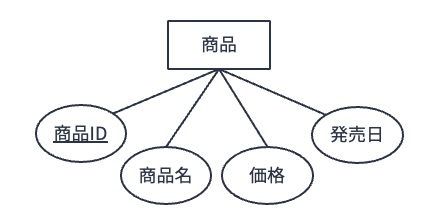
\includegraphics[width=0.7\textwidth]{figure/er-model/product-entity.jpg}
    \caption{実体型「商品」の実体関連図}
    \label{fig:product_entity}
\end{figure}

\begin{notebox}{「一意に識別できる」とは？}
実体や関連の定義において「一意に識別（特定）できる」という言い回しが頻繁に使われます．
「事柄Xが（ある集合内において）一意に識別できる」とは「集合内に事柄Xとまったく同じものがなく，集合の中からXをピタリと特定できる」という意味です．

例えば実体型「商品」において「商品ID」が主キーとなっている場合，商品集合内の各商品は「（商品IDをもって）一意に識別できる」と言えます．
これは「商品IDを見れば，（他の商品と区別して）ある商品を唯一1つに絞り込むことができる」という意味になります．
言い換えれば，実体集合「商品」においては，まったく同じ「商品」は存在しない（してはいけない）という意味になります．
\end{notebox}


\subsection{関連}
\strong{関連（relationship）}とは，複数の実体間のつながりを表します\footnote{「関連」と「関係」は混同しやすいが異なる概念なので注意すること．「関連（relationship）」は実体関連モデルにおける概念で，複数の実体間のつながりを表します．一方，「関係（relation）」は数学や関係データベース上の概念で，集合の直積の部分集合を意味します．}．
例えば，Amazonなどのショッピングサイトでしばしば提供されている，欲しい（購入希望の）商品をリスト化しておく「ウィッシュリスト（お気に入り）」機能について考えてみましょう．
これを実体関連モデルで表現するならば，実体「ユーザ」と実体「商品」の間に「お気に入り」という関連を定義することができます．
関連は，結びつく実体（ユーザや商品など）が存在して初めて意味を持ちます．
例えば，先に挙げた関連「お気に入り」について，お気に入り（として登録する）という行為は行為主体であるユーザと行為対象である商品がそろって初めて定義できます．

同じ種類の関連の集合は\strong{関連集合（relationship set）}と呼ばれます．
例えば，先の「お気に入り」の例では，
\begin{itemize}
\item ユーザAが商品Xをお気に入り登録したこと
\item ユーザBが商品Yをお気に入り登録したこと
\end{itemize}
など，個々のユーザが何かをお気に入り登録したという行為の集合が関連集合「お気に入り」となります．
% 関連集合内の各関連は，それとつながっている複数の実体によって「一意に識別」されます．
% 言い換えると，ある関連はそれとつながっている実体の主キーの値が指定されたとき，一意に識別されなければなりません．
% これは非常に重要かつ分かりにくいポイントです．

関連型も属性を持つ場合があります（属性がないこともあります）．
例えば，先の関連型「お気に入り」の例であれば，サイトにお気に入りを登録した「登録日」などが属性として考えられます．

Peter Chenの記法では実体関連図において，
\begin{itemize}
\item 関連型はひし形
\item その属性は楕円
\end{itemize}
で表現されます．
関連型とその属性は線で結び，関連型はつながりのある実体型と線で結びます．

図\ref{fig:wishlist_relationship}は，実体型「ユーザ」「商品」，および関連型「お気に入り」を実体関連図として表現したものです．
\figure[htb]
    \centering
    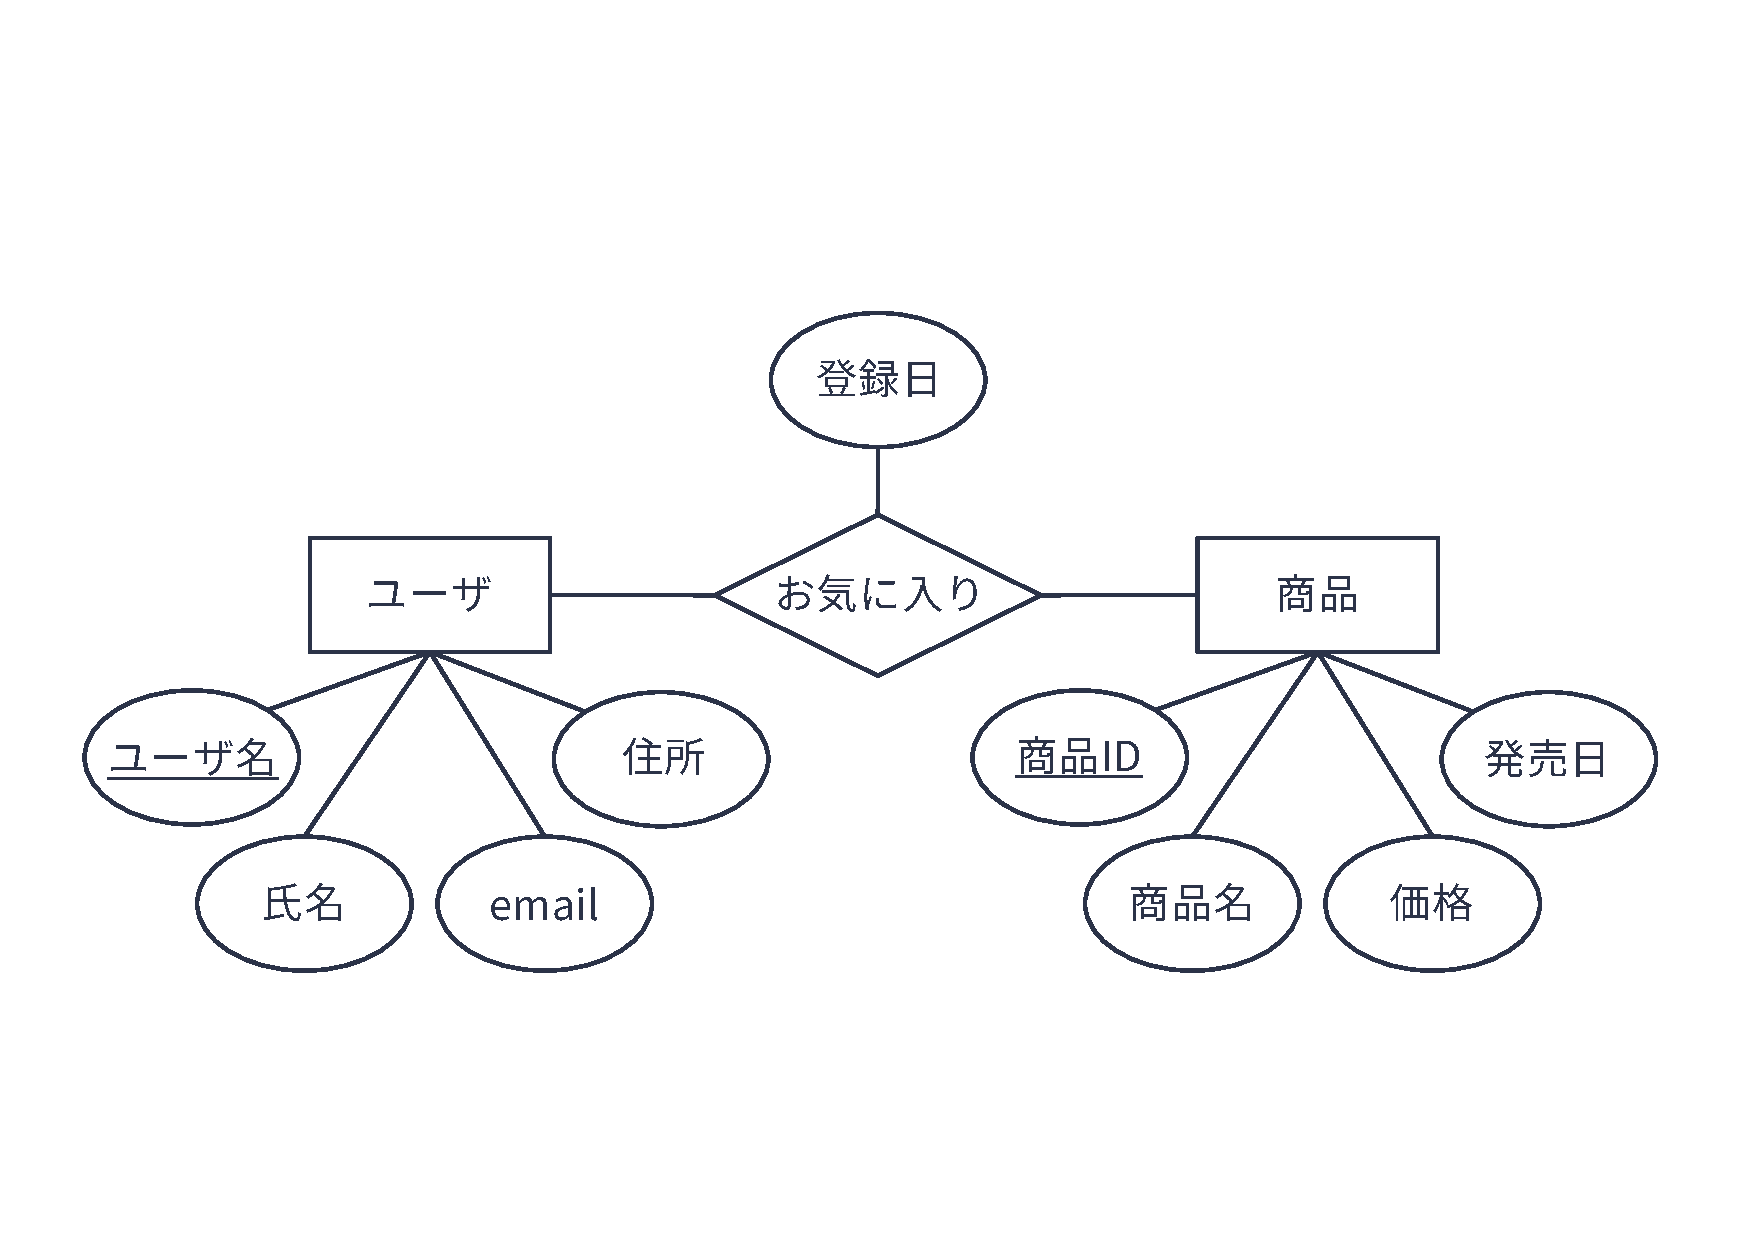
\includegraphics[width=0.85\textwidth]{figure/er-model/wishlist-relationship.pdf}
    \caption{実体型「ユーザ」「商品」と関連型「お気に入り」の実体関連図}
    \label{fig:wishlist_relationship}
\endfigure

実体は実体集合内で一意に識別できる必要があると述べましたが，関連も関連集合内で一意に識別できる必要があります．
もう少し具体的に言うと，ある関連はそれとつながっている実体の主キーの値が指定されたとき，一意に識別されなければなりません．
実際，実体関連モデルにおける関連は，数学的には「実体の主キーの組み合わせ」として扱われます．
これは非常に重要ですが，分かりにくいポイントでもあるので，例を挙げて考えてみましょう．

図\ref{fig:er_model_elements}は，上の実体関連図に示したモデルの実体および関連（つまり実体集合および関連集合の要素）の例を図示したものです．
ベン図において，点は各集合の要素（つまり実体や関連）を表しています．
実体「ユーザ」「商品」の点の下に書かれた値は，ある実体の主キーの値を示しています．
また，関連「お気に入り」の下に書かれた値は，各関連につながる実体の主キーの値のペアを示しています．
例えば，真ん中の\graybox{(U1,P1)}の点は，ユーザ\graybox{川澄}（主キーは\graybox{U1}）が商品\graybox{はーいお茶}（主キーは\graybox{P1}）をお気に入り登録したことを表しています．
このように，一つ一つの関連「お気に入り」は実体「ユーザ」と「商品」の主キーのペアで表現されます．
それによって，「ユーザ」の主キーと「商品」の主キーの値が指定されれば．どの関連「お気に入り」かを一意に識別できるようになっています．
すでに説明したように，関連集合の要素は一意に識別できる必要があります．
そのため，図の赤バツ印の箇所のように，ユーザ\graybox{川澄}が商品\graybox{はーいお茶}を2回目のお気に入り登録することできません．
関連集合は「集合」であるため，\graybox{(U1,P1)}のような同じ値の要素を複数持つことはできないのです．
この実体関連モデルでは，ユーザは同じ商品に対するお気に入りを1回分しか登録できないことになります．
あるユーザの同じ商品に対する複数回のお気に入りを別々に扱いたい場合は，モデリングを工夫する必要があります（これについては，後ほど説明します）．
\figure[htb]
    \centering
    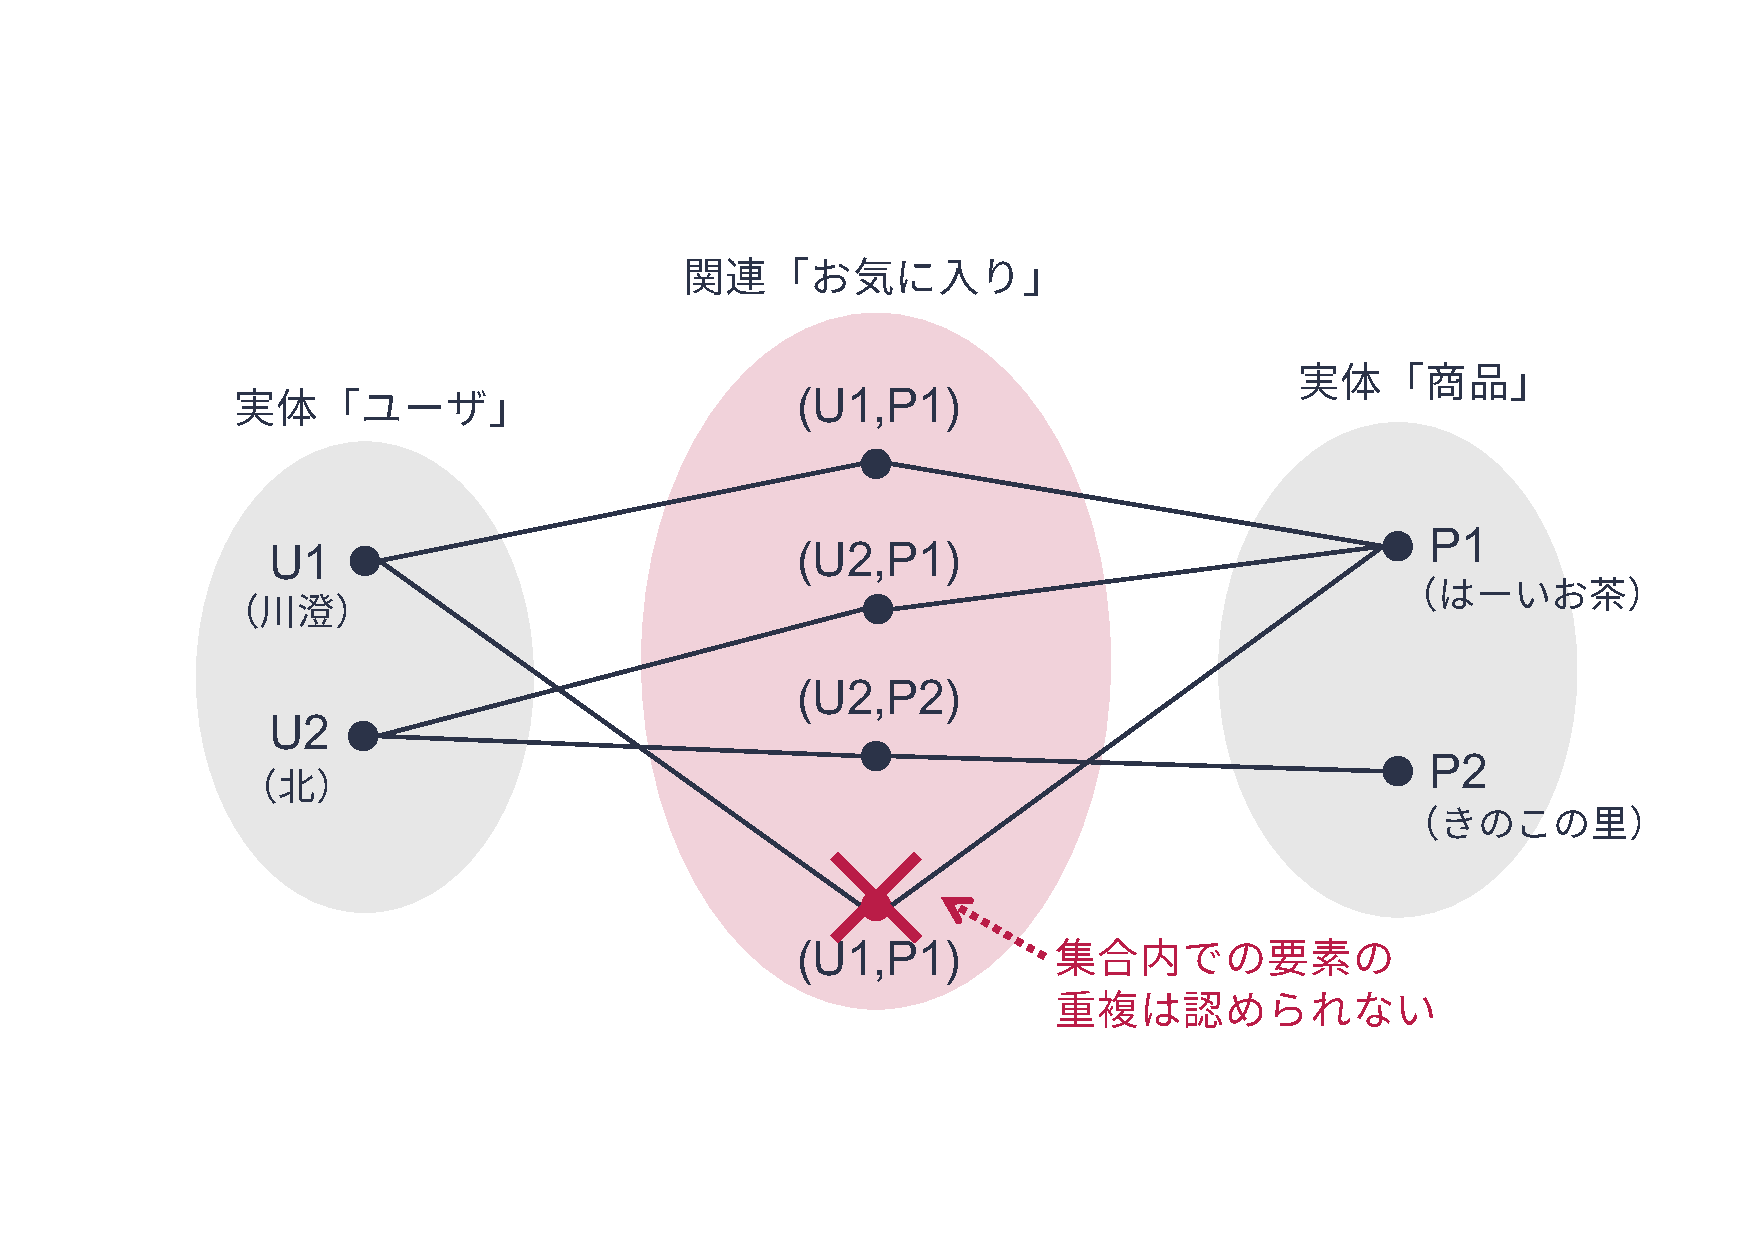
\includegraphics[width=0.85\textwidth]{figure/er-model/er-model-elements.pdf}
    \caption{実体型「ユーザ」「商品」と関連型「お気に入り」の実体集合および関連集合の要素の例}
    \label{fig:er_model_elements}
\endfigure



\subsection{役割の明示}
ある大学ではデータベースを用いた学生情報の管理を検討しています．
さて，この大学ではどの学生も
\begin{itemize}
\item 自分の面倒を見てくれる「先輩」学生
\item 面倒を見てあげる必要のある「後輩」学生
\end{itemize}
が割り当てられているとします．
このような状況を実体関連モデルで表現することを考えてみましょう．

与えられた条件をふまえて
\begin{itemize}
\item 実体型として「先輩学生」と「後輩学生」，
\item 先輩学生と後輩学生とのつながりを表す関連型として「世話」
\end{itemize}
を定義したとしましょう．
この定義に従ってデータを管理しようとすると，面倒なことが起きます．

例えば，山畑滝子さんという学生には，川澄桜子さんという先輩と田辺通さんという後輩がいたとしよう．
この状況を先に定義した実体関連モデルで考えてみると，図\ref{fig:er_model_without_role}のように，\graybox{山畑滝子}という唯一無二の実体が実体集合「先輩学生」と実体集合「後輩学生」のそれぞれの要素に現れてしまいます．
検討しているデータベースでは学生情報を管理したいので，2つの実体集合に同じ情報が二重に登場するのは冗長で望ましくありません．
先の実体関連モデリングは適切ではなかったのです．
\begin{figure}[htb]
    \centering
    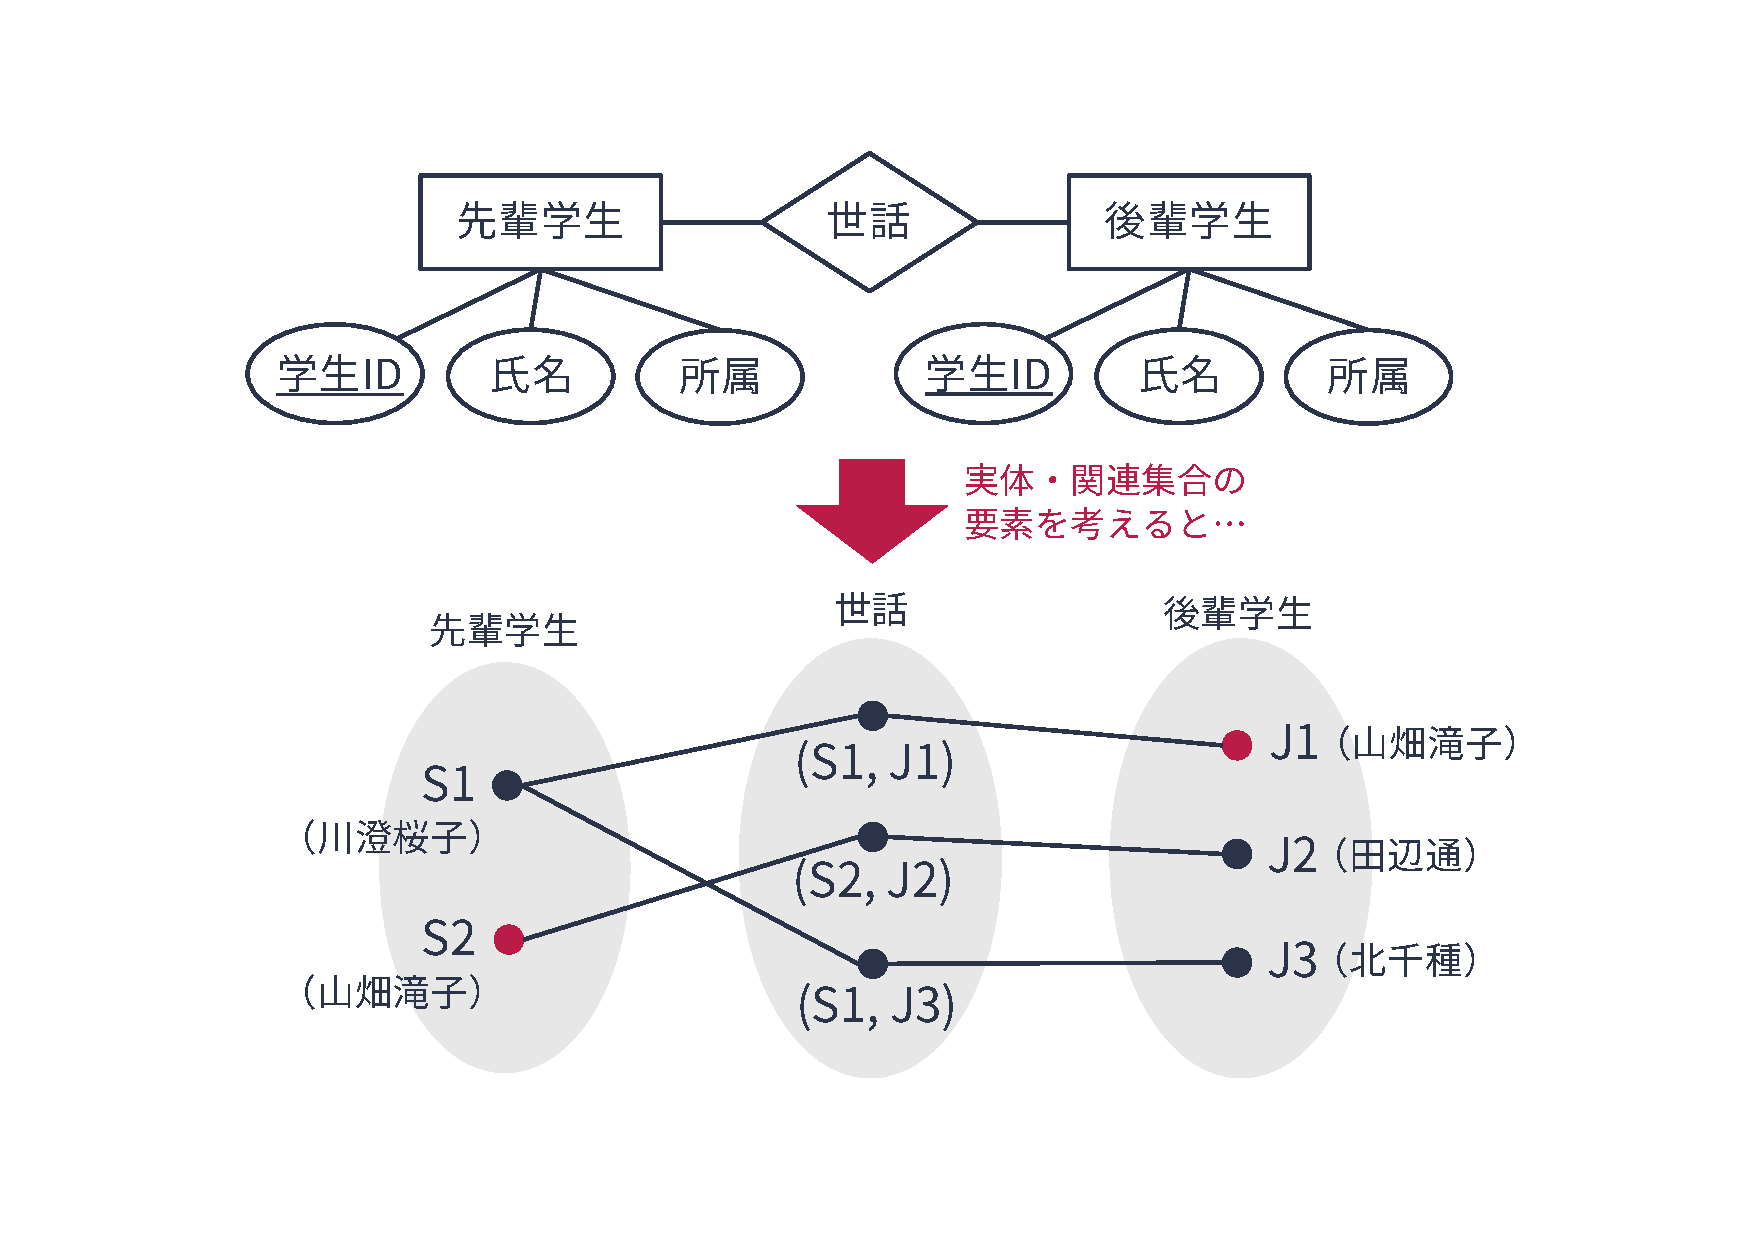
\includegraphics[width=0.8\textwidth]{figure/er-model/er-model-without-role.pdf}
    \caption{役割を明示しない実体関連図の例．分かりやすさのために，要素の隣には属性「名前」の値を記載している．}
    \label{fig:er_model_without_role}
\end{figure}

先輩学生であっても後輩学生であっても学生は学生です．
どちらの実体も実体型「学生」とその他の関連型のみで学生間の先輩後輩関係を表現できないのでしょうか．

同一の実体型間に関連型が存在するケースでは，枝の上に役割を明示することで対応します．
先の例では，図\ref{fig:er_model_with_role}のように，実体型「学生」と関連「世話」の間に
\begin{itemize}
\item 先輩関係を表す直線
\item 後輩関係を表す直線
\end{itemize}
を別々に引き，直線が意味する役割を明示します（つまり2本の線を引く）．
こうすることで，学生の概念を実体型「学生」だけに集約ができ，かつ先輩後輩の関係を表現できるようになります．
\begin{figure}[htb]
    \centering
    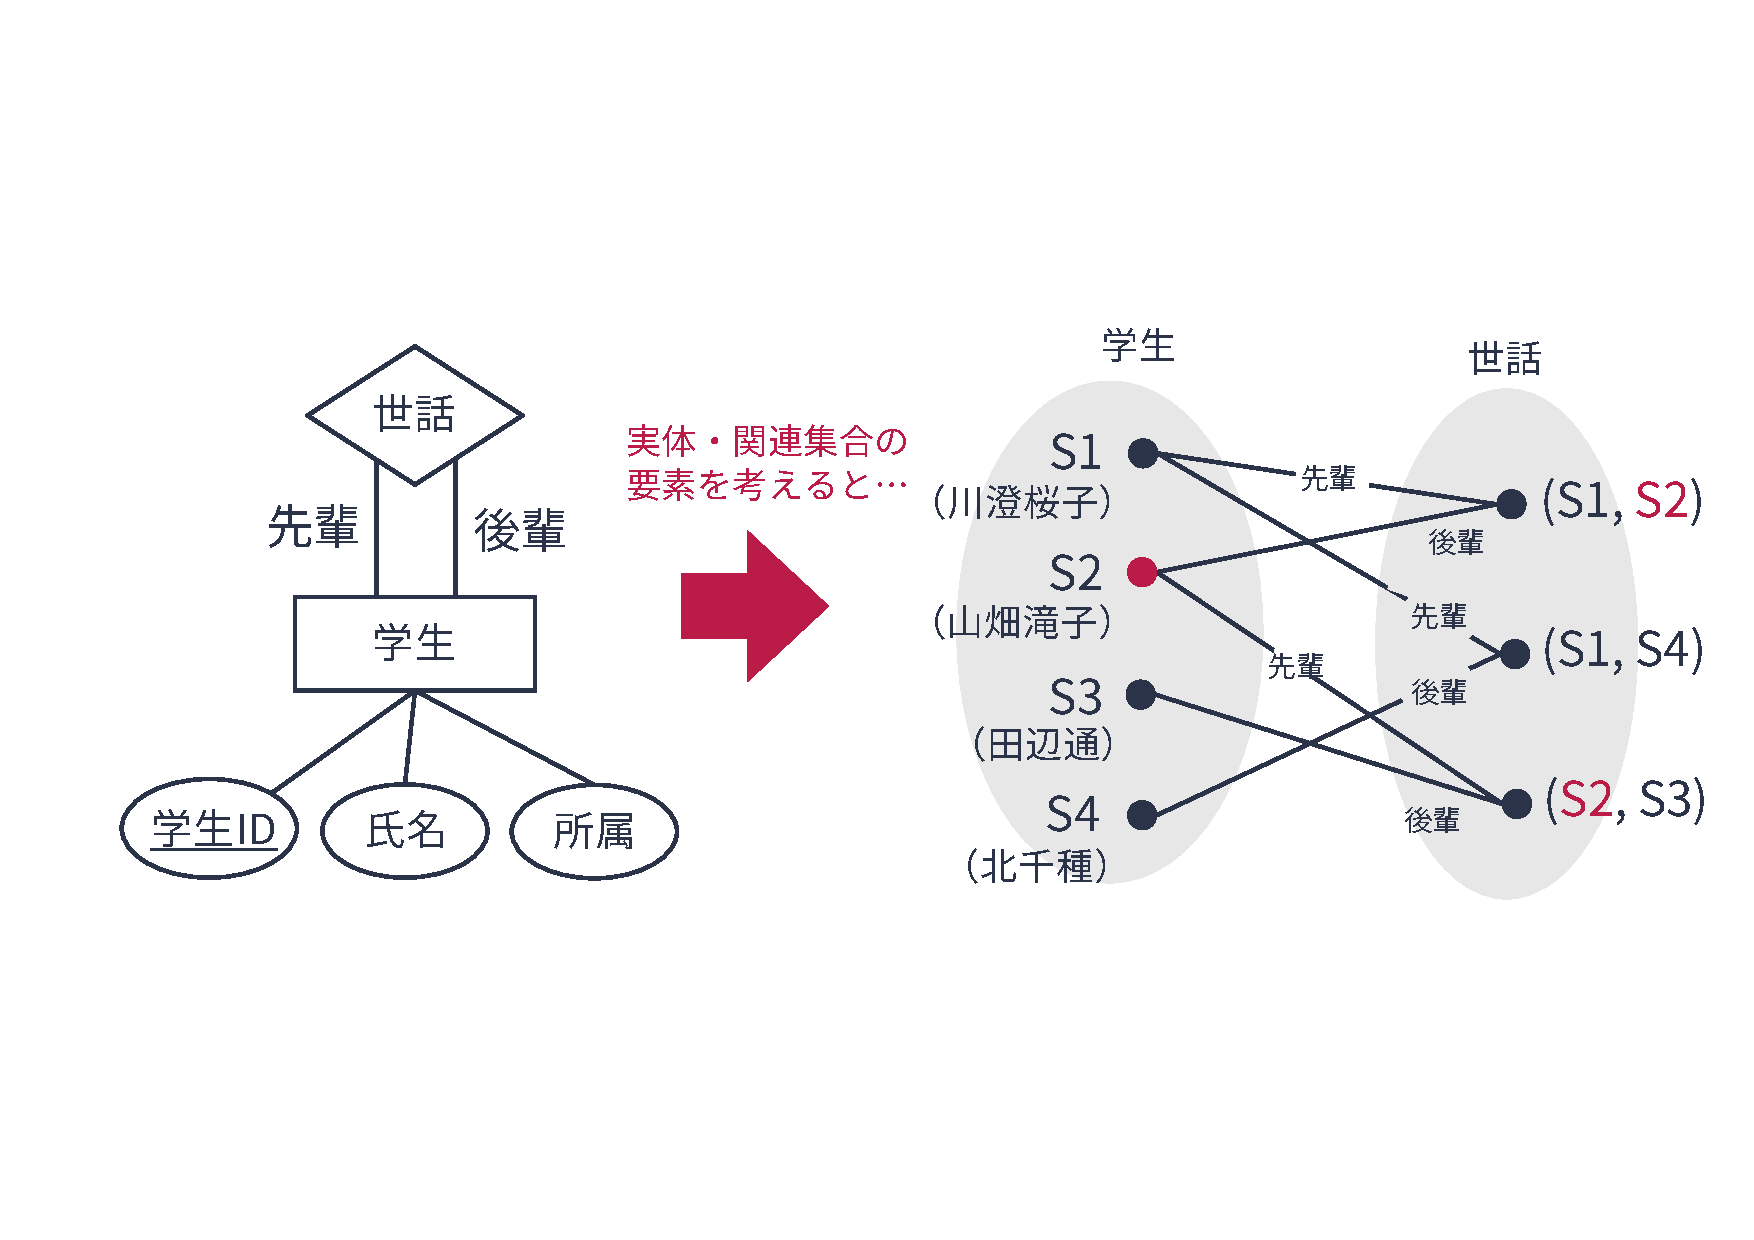
\includegraphics[width=1.0\textwidth]{figure/er-model/er-model-with-role.pdf}
    \caption{役割を明示した実体関連図の例}
    \label{fig:er_model_with_role}
\end{figure}


\begin{notebox}{実体，関連，属性を見分ける経験則}
与えられたシナリオから実体関連図を作成しようとしても，何を実体として何を関連として見なすか，どれを属性として見なすか，迷うことがあるでしょう．
実体関連モデルを提唱したPeter Chenは自身が発表した論文\cite{Chen1997}において，以下のような経験則を提案しています．
\begin{itemize}
\item 普通名詞: 実体型
\item 固有名詞: 実体
\item 他動詞: 関連型
\item 自動詞: 属性
\item 形容詞: 実体の属性
\item 副詞: 関連の属性
\end{itemize}
以上の経験則は当てはまらないこともありますが，一定の目安にはなります．
実体関連モデルを習い始めたばかりの人は参考にしてみてください．
\end{notebox}


\section{実体関連モデルにおける一貫性制約}
関係データモデルでは，対象となるデータが持つべき条件としてドメイン制約やキー制約といった一貫性制約を定義します．
実体関連モデルにおいても，データが持つべき一貫性制約を表現・設定する方法がいくつか用意されています．
以下では，実体関連モデルにおける代表的な一貫性制約である\strong{参加制約}，\strong{多重度制約}，\strong{キー制約}について説明します．

\subsection{参加制約}
図\ref{fig:er_model_elements2}を見てみましょう．
図\ref{fig:er_model_elements2}は，あるショッピングサイトにおける商品の「お気に入り」に関する実体型および関連型の要素を示したものです（図\ref{fig:er_model_elements}と似ていますが，問題のあった関連（お気に入り\graybox{(U1,P1)}の2つ目）を取り除き，商品\graybox{P3}を追加しています）．
図の実体型「商品」に注目すると，どの実体「ユーザ」とも関連を持たない実体「商品」\graybox{タケノコの里（P3）}が存在していることが分かります．
これは，誰も商品\graybox{P3}の購入を希望していないことを意味します．
\figure[htb]
    \centering
    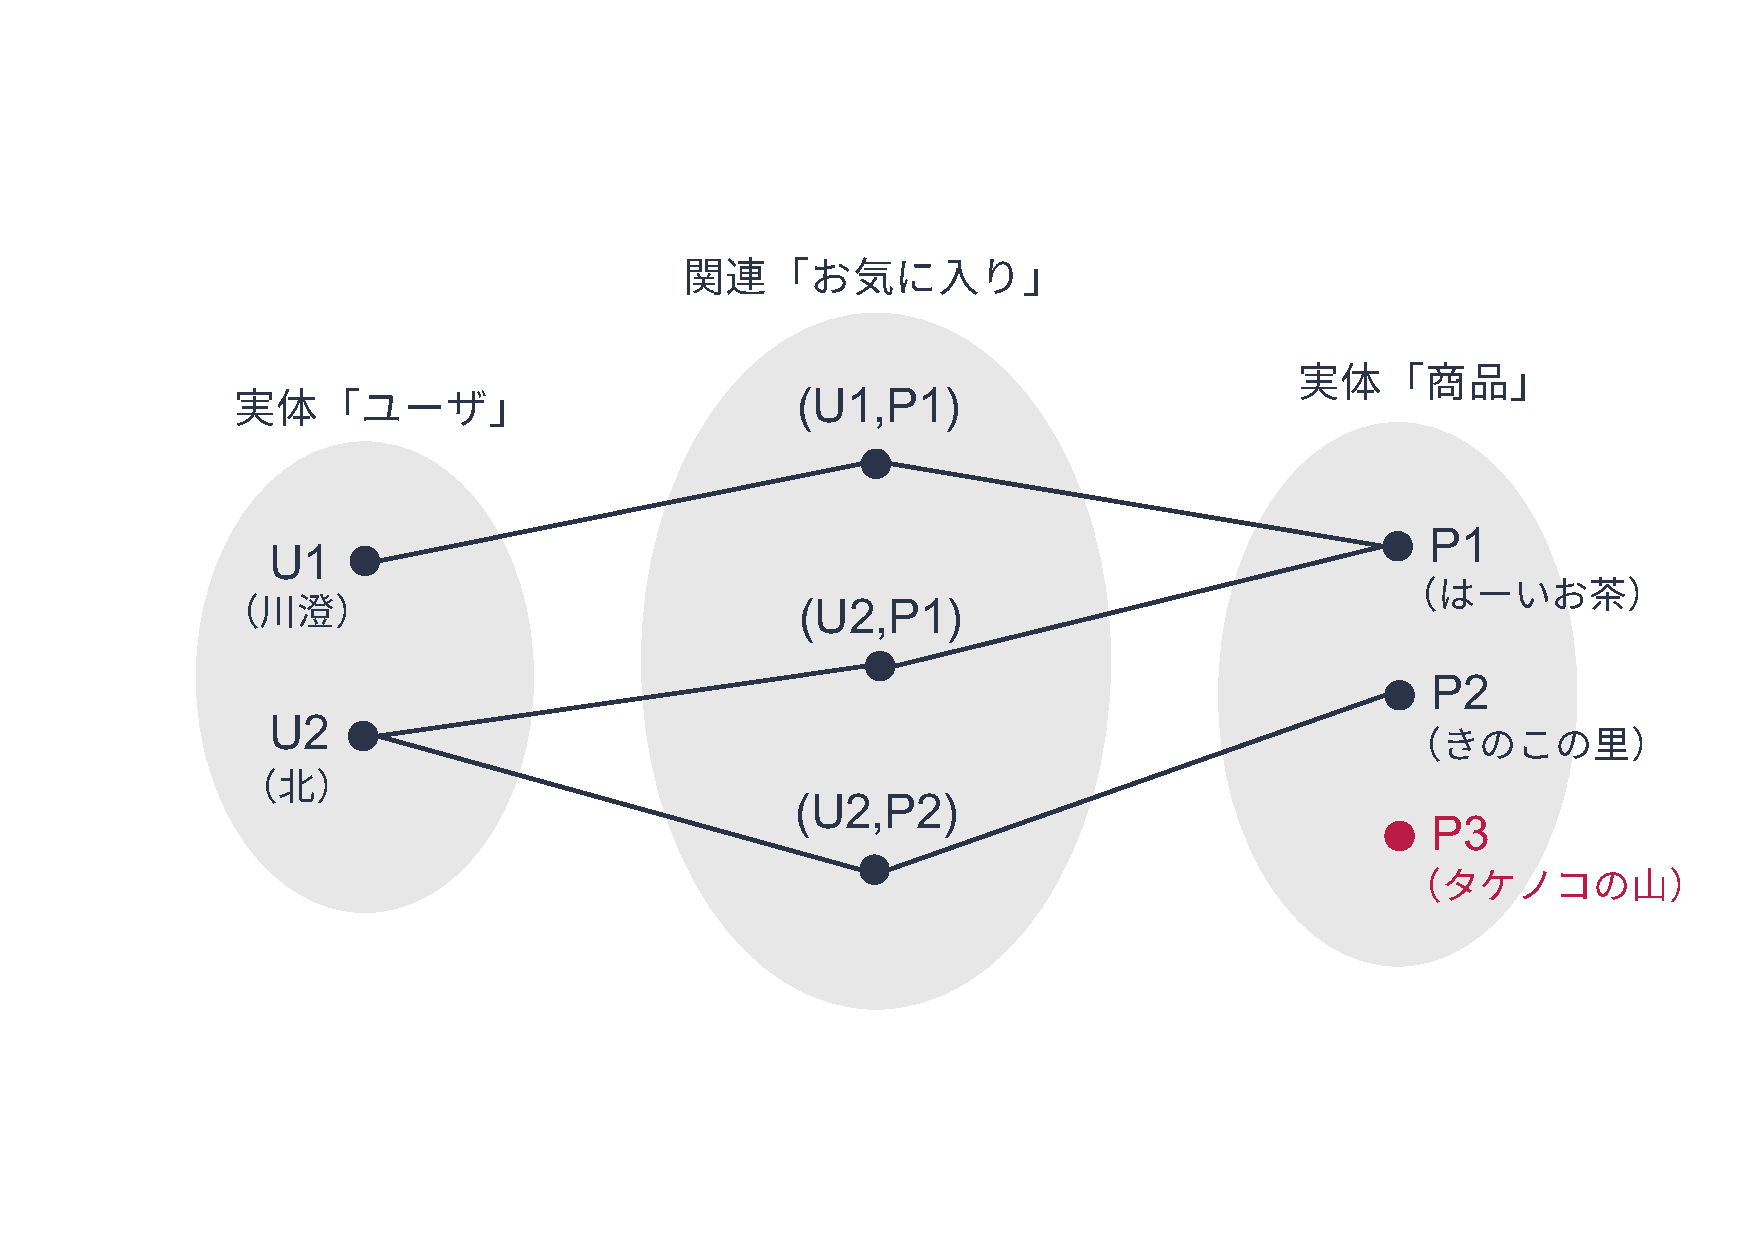
\includegraphics[width=0.85\textwidth]{figure/er-model/er-model-elements2.pdf}
    \caption{どの実体「ユーザ」とも関連を持たない実体「商品」が存在している例．}
    \label{fig:er_model_elements2}
\endfigure

実体関連図上で実体型$E_1$と実体型$E_2$が関連型$R$でつながっているときに，モデリングの対象としている問題設定によっては，実体集合$E_1$のすべての要素が関連集合$R$の要素とつながっていてほしい場合があります．
このようなケースを，$E_1$の$R$への参加は\strong{全体的}であると呼びます．

逆に$E_1$の集合内の全要素が関連集合$R$の全要素とつながっている必要がない場合，$E_1$の$R$への参加は\strong{部分的}であると呼びます．
実体型$E$の関連型$R$への参加が「部分的」であるときは，実体関連図上では$E$と$R$の間の直線を\strong{細線}にすることによって表現します．
例えば，先のショッピングサイトの図\ref{fig:er_model_elements2}のケースの場合，誰もお気に入りをしていない商品が存在しても構わないため，実体型「商品」は関連型「お気に入り」への参加は「部分的」としています．
このように，ある実体型のある関連型への参加（つながり）が全体的か部分的かを定める制約を\strong{参加制約（participation constraint）}と呼びます．

実体型$E$の関連型$R$への参加が「全体的」であるとき，実体関連図上では$E$と$R$の間の直線を\strong{太線}にすることによって表現します．
例えば，先のショッピングサイトの例において，実体型「商品」の関連型「お気に入り」への参加が「全体的」であるとするときは，図\ref{fig:participation_constraint}のような実体関連図にします．
\figure[tb]
    \centering
    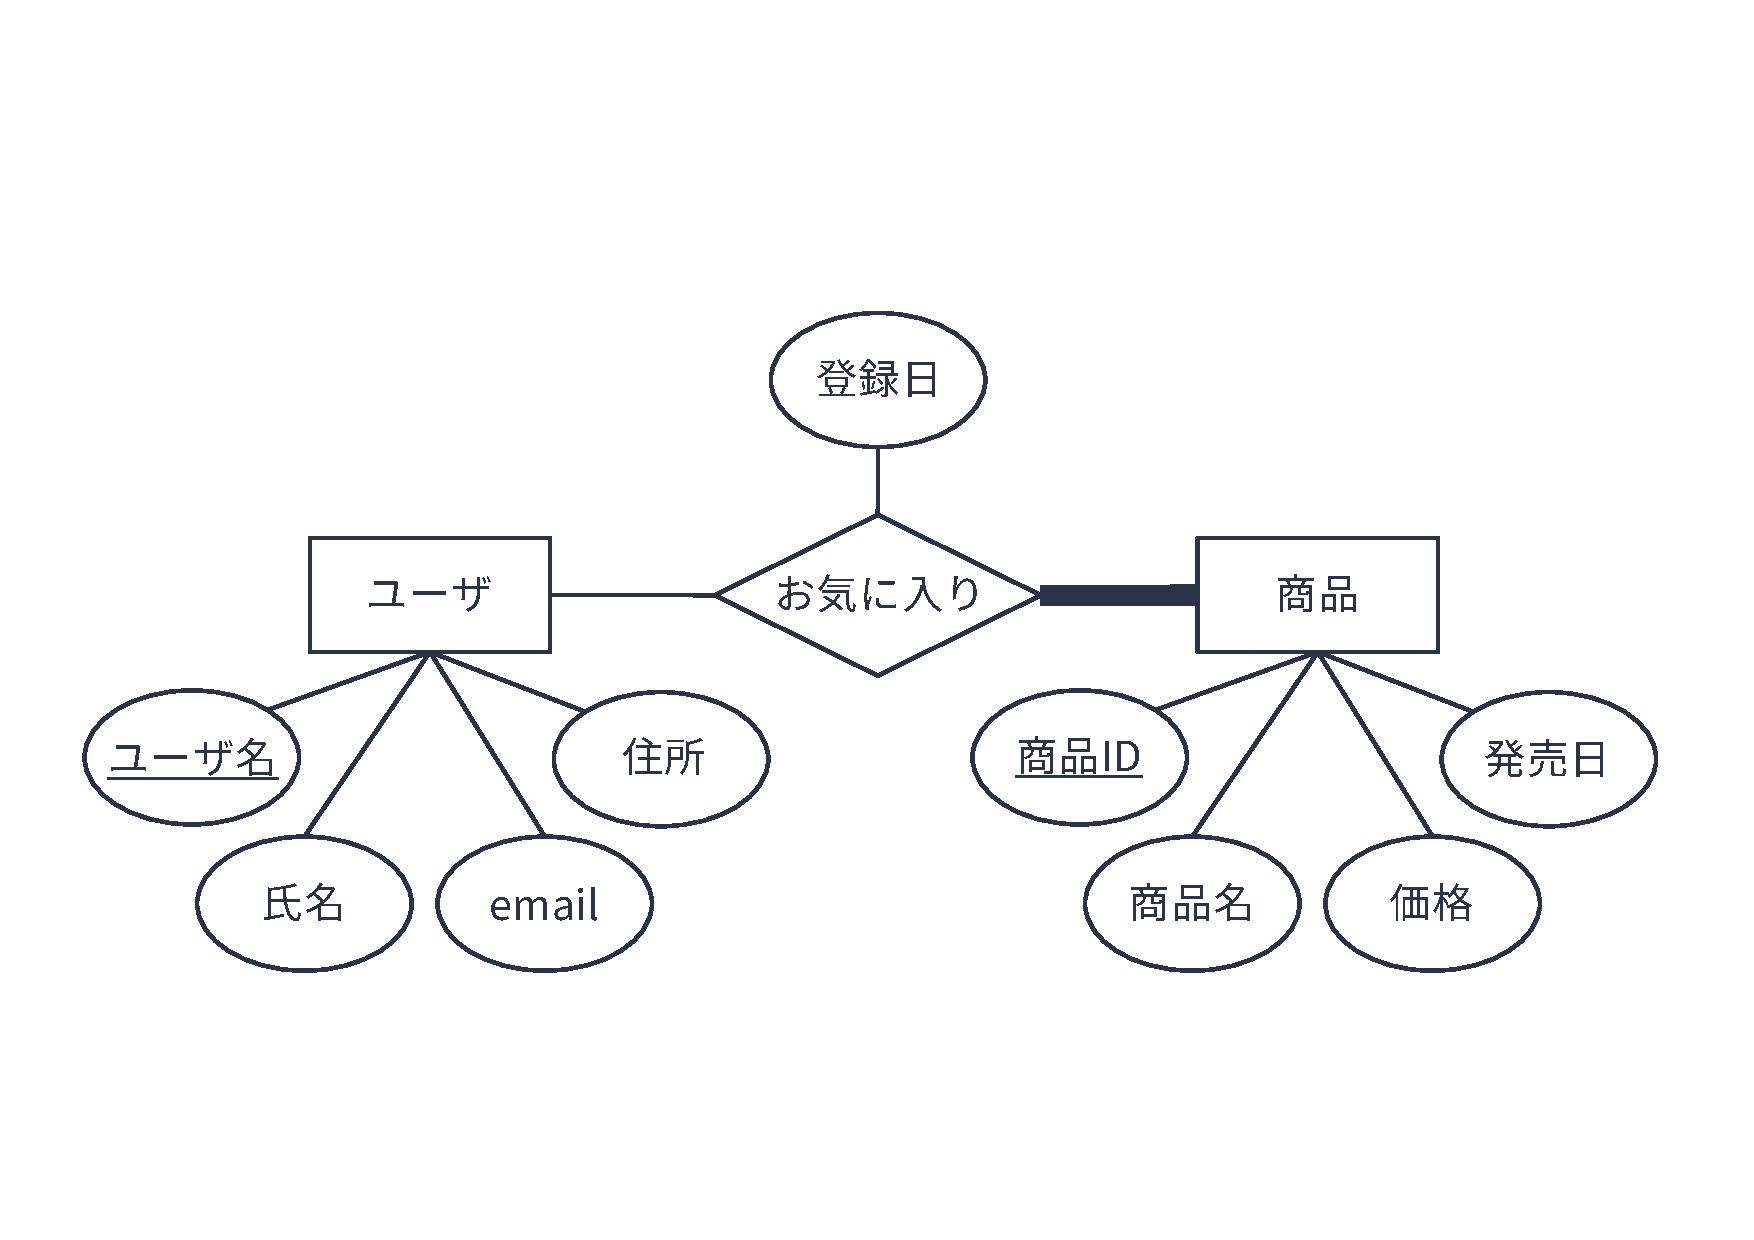
\includegraphics[width=1.0\textwidth]{figure/er-model/participation-constraint.pdf}
    \caption{参加制約の例}
    \label{fig:participation_constraint}
\endfigure
図\ref{fig:participation_constraint}のように定義することで，どの実体「商品」も必ずいずれかの関連「お気に入り」とつながっている必要があります．
逆に，図では実体「ユーザ」は関連「お気に入り」への参加が「部分的」となっているため，つまりお気に入り登録したことがないユーザが存在することを許しているということにもなります．


\subsection{多重度制約}
ショッピングサイトの例に戻りましょう．
図\ref{fig:er_model_elements3}は，お気に入り登録に加えて，各商品がどのメーカーによって製造されたかの情報についても管理する実体関連モデルを設計し，それに基づき実体集合「ユーザ」「商品」「メーカー」および関連集合「お気に入り」「製造」の要素を図示したものです．
\figure[htb]
    \centering
    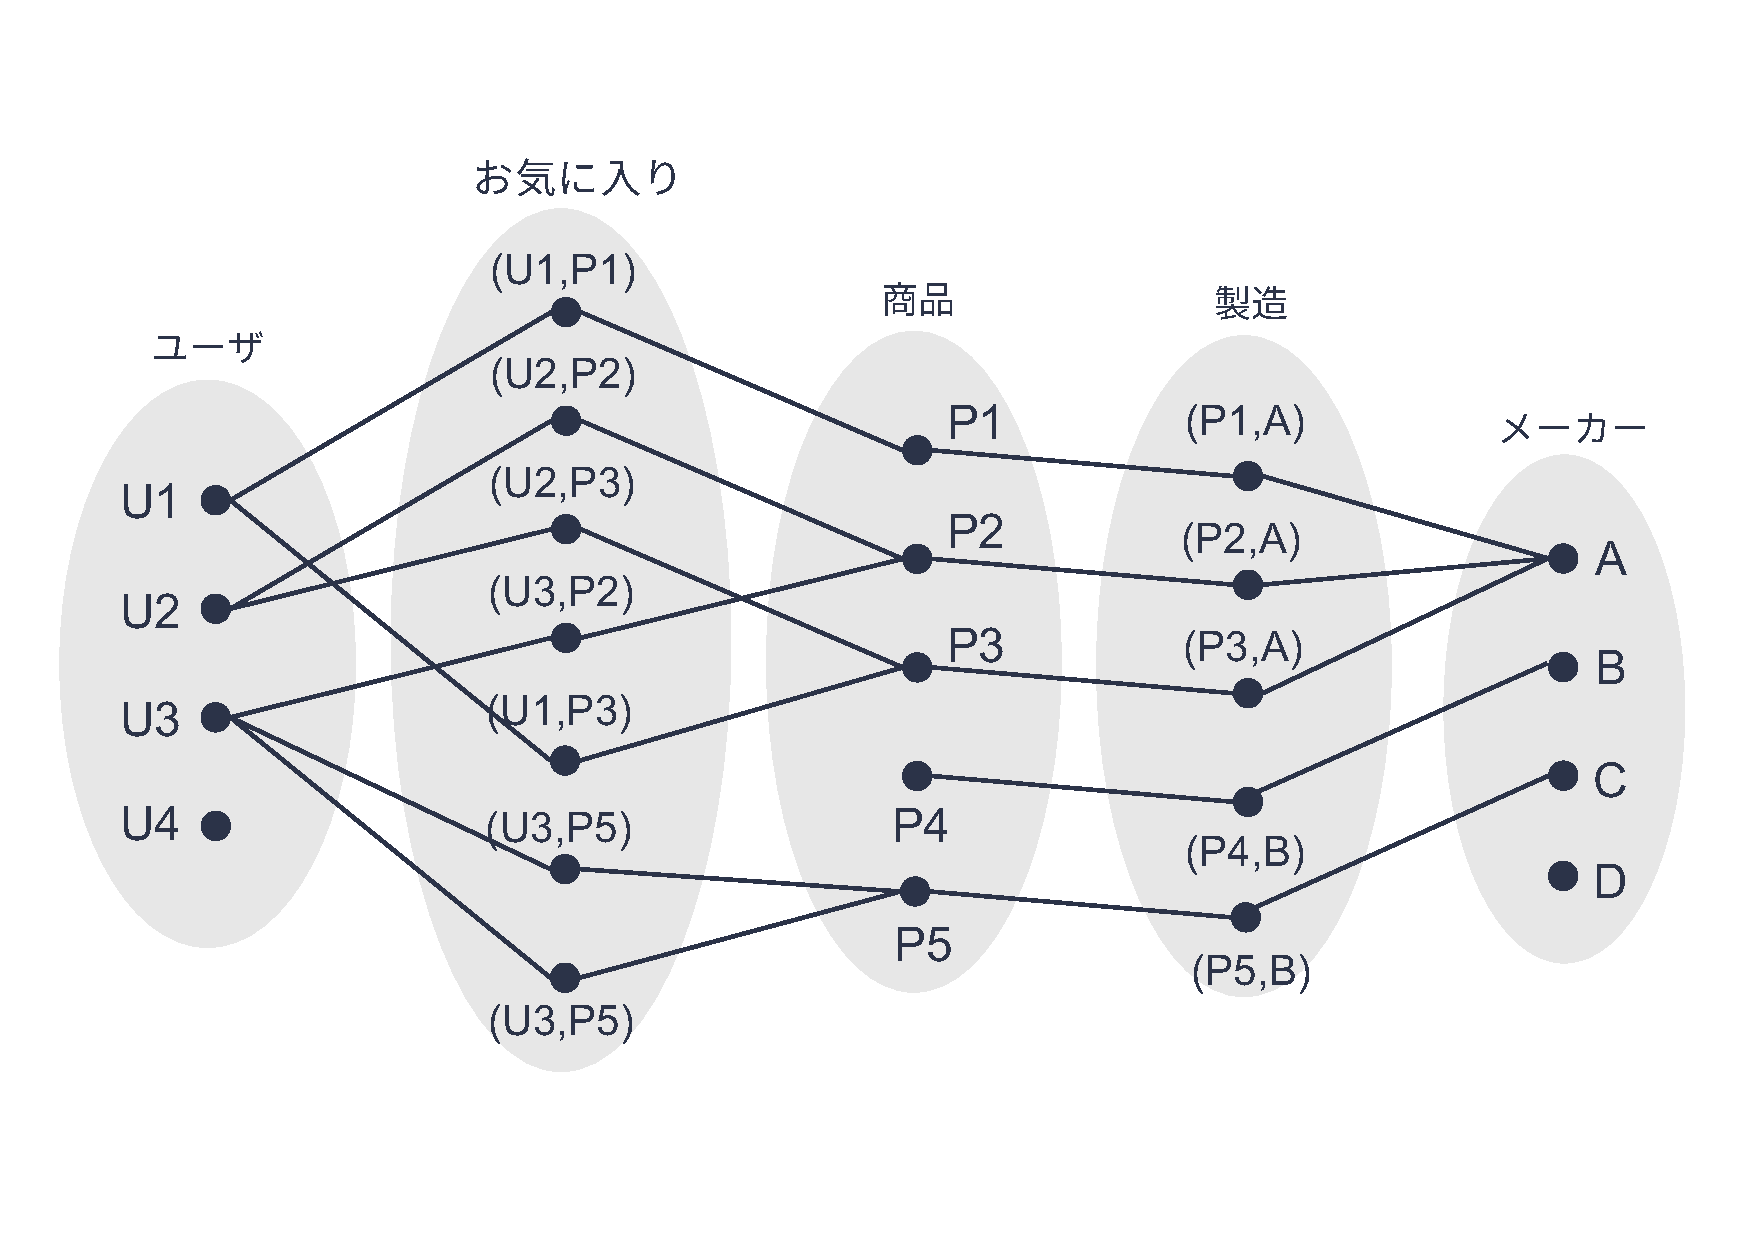
\includegraphics[width=1.0\textwidth]{figure/er-model/er-model-elements3.pdf}
    \caption{実体「メーカー」と関連「製造」も加えた実体関連図の要素の例．}
    \label{fig:er_model_elements3}
\endfigure
（図が物語っていることがすべてであるとすると）この図からは，以下のことが分かります．
\begin{enumerate}
\item ユーザは複数の商品をお気に入り登録することができる
\item 商品は複数のユーザからお気に入り登録されてもよい
\item ユーザの中には商品をお気に入り登録をしない者がいてもよい
\item 商品の中にはユーザにお気に入り登録されないものがあってもよい
\item 商品は必ず1つのメーカーによって製造される（複数のメーカーが合同で1つの商品を製造することはない）
\item メーカーは複数の商品を製造する
\item メーカーの中には商品を製造していないところがあってもよい
\end{enumerate}

以上のことを実体関連図上で表現してみましょう．
上記項目のうち，項目3，4，5，7については参加制約に関する事柄です．
すなわち，
\begin{itemize}
\item 実体型「ユーザ」の関連型「お気に入り」への参加制約は「部分的」
\item 実体型「商品」の関連型「お気に入り」への参加制約は「部分的」
\item 実体型「商品」の関連型「製造」への参加制約は「全体的」
\item 実体型「メーカー」の関連型「製造」への参加制約は「部分的」
\end{itemize}
となります．

一方，項目1，2，6（そして5）は，ある実体（要素）から見たときに，ある関連を通じて異なる実体（要素）と「いくつ」つながることが許されるかという制約を示しています．
このように，ある関連に対して対応づけ可能な実体の数を\strong{多重度（cardinality）}\footnote{Cardinalityは多重度と呼ばれることもあるが，語源からすると「濃度」が正しい訳語とする説がある．}と呼びます．
また，多重度に関する制約を\strong{多重度制約（cardinality constraint）}と呼びます．

実体間の関連は「1対1」「1対多」「多対多」のいずれかとなります．
例えば，上記図においては
\begin{itemize}
\item 関連「お気に入り」はユーザと商品の「多対多」関連（項目1および2）
\item 関連「製造」はメーカーと商品の「1対多」関連（項目5および6）
\end{itemize}
と見なせます．

実体関連図において，多重度は以下のように表現します．
\begin{itemize}
\item 1対1関連: 関連型から実体型に引かれた線をすべて矢印線にする
\item 1対多関連: 関連型から「1」に対応する実体型に引かれた線のみを矢印線にする
\item 多対多関連: 関連型から実体型に引かれた線をすべて直線にする（矢印は加えず，そのままにする）
\end{itemize}
図\ref{fig:er_model_elements3}の内容を踏まえて実体関連図を設計すると，図\ref{fig:cardinality_constraint}のようになります．
例えば，関連型「お気に入り」から実体型「ユーザ」への線は直線に，関連型「製造」から実体型「メーカー」への線は矢印線になります．
\begin{figure}[htb]
    \centering
    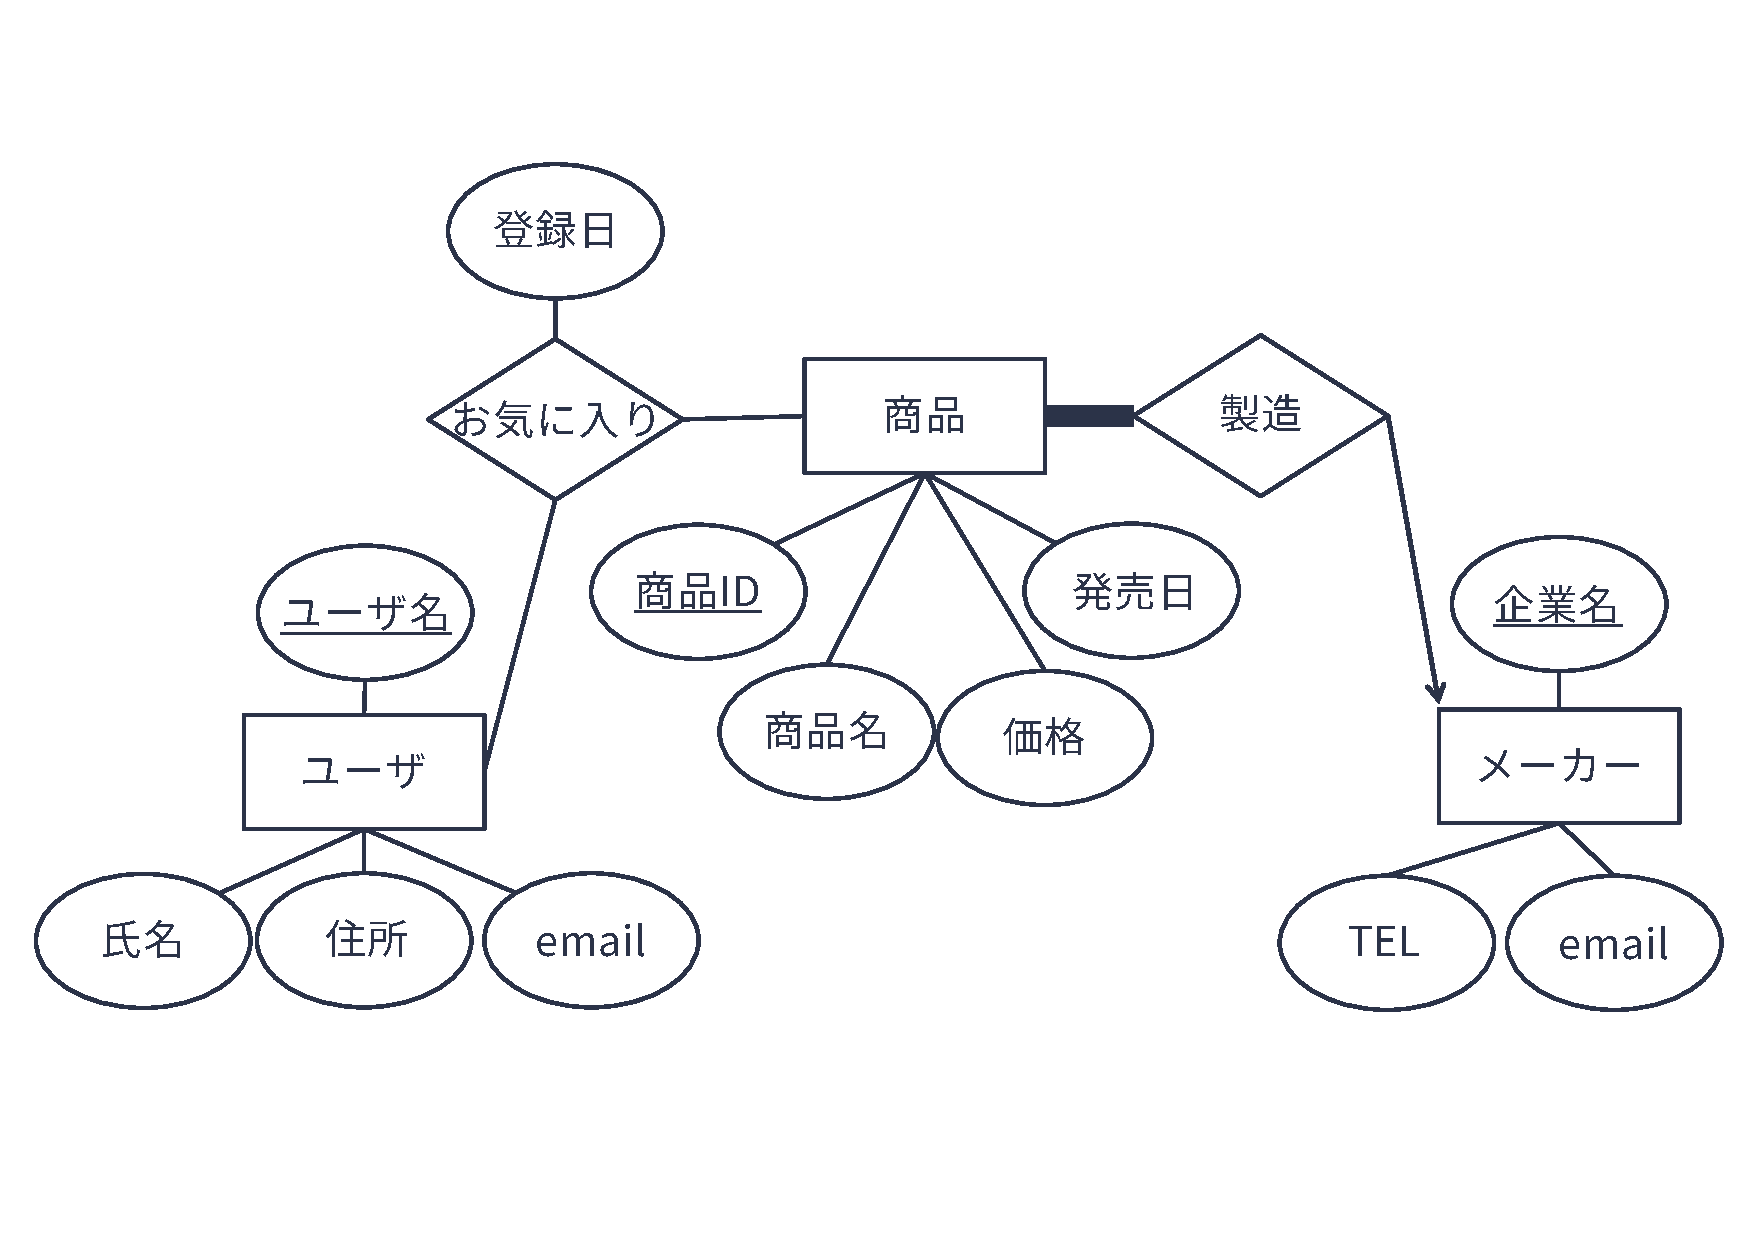
\includegraphics[width=1.0\textwidth]{figure/er-model/cardinality-constraint.pdf}
    \caption{多重度制約を表現した実体関連図の例．}
    \label{fig:cardinality_constraint}
\end{figure}


\subsection{キー制約}
実体関連モデルにおける\strong{キー制約（key constraint）}とは，キーとして指定された属性はキーとしての役割を必ず果たす必要があるという制約です．
例えば，実体型「学生」の属性「学籍番号」が主キーとして設定された場合，指定された学籍番号によって実体「学生」は一意に特定できなければなりません．
また，学籍番号に重複は許されません．
実体型の説明で述べたように，実体関連図において主キーとなる属性には下線を引きます．

\subsubsection{弱実体と部分キー}
ショッピングサイトの例に戻りましょう．
ショッピングサイトを利用する際，自分のユーザ名を使ってログインをしたものの，購入した商品の送り先を同居する家族の名前にしたい，というケースを考えましょう．
このようなケースに対応するため，サイト運営者は先ほど示した図\ref{fig:cardinality_constraint}の実体関連図を改善して，
\begin{itemize}
\item 実体型「家族」を追加
\item 実体「ユーザ」と実体「家族」が同居関係にあることを示すために，関連型「同居」を追加
\end{itemize}
すること検討しているとしましょう．
この際，「家族」にはユーザ名は割り振られず，家族の誰かに商品を送るときは，その家族のユーザがサイトにログインをして手続きをすることを想定してください．

このようなケースは，\strong{弱実体}という特殊な概念を用いて実体関連図を設計することがあります．
自身がもつ属性だけでは主キーを構成できない特殊な実体集合を\strong{弱実体集合（weak entity set）}と呼びます．
弱実体を特定する上で，それと関連している実体のことを\strong{所有実体（owner entity）}と呼びます．
弱実体と所有実体をつなげる関連を\strong{弱関連（weak relationship）}と呼びます．
また，弱実体を一意に特定するために，所有実体の主キーとセットにして使われる弱実体の属性を\strong{部分キー（partial key）}と呼びます．
所有実体と部分キーが決まって初めて，弱実体集合の中にある弱実体を一意に特定できるようになります．

実体関連図において，弱実体型は二重線の矩形，弱関連型は二重線のひし形で表現します．
また，部分キーには点線を引きます\footnote{書籍によっては部分キーには下線を引くと書かれている場合もありますが，本書では主キーと分かりやすく区別するために点線を用います}．

先の家族を扱うケースについて，弱実体と弱関連の概念を用いても実体関連図を作成すると，図\ref{fig:weak_entity}のようになります．
図\ref{fig:weak_entity}においては，
\begin{itemize}
\item 実体「家族」が弱実体（「氏名」が部分キー）
\item 実体「ユーザ」が（弱実体「家族」に対する）所有実体
\item 関連「同居」が弱関連
\end{itemize}
となります．
図中では，弱実体型「家族」は「氏名」「続柄」のみを属性として持っています．
なお，「氏名」は部分キーであり，弱実体型「家族」の主キーに設定していません．
主たるユーザがいてこその弱実体「家族」であり，「家族」を独立して管理する意味がないからです．
\begin{figure}[tb]
    \centering
    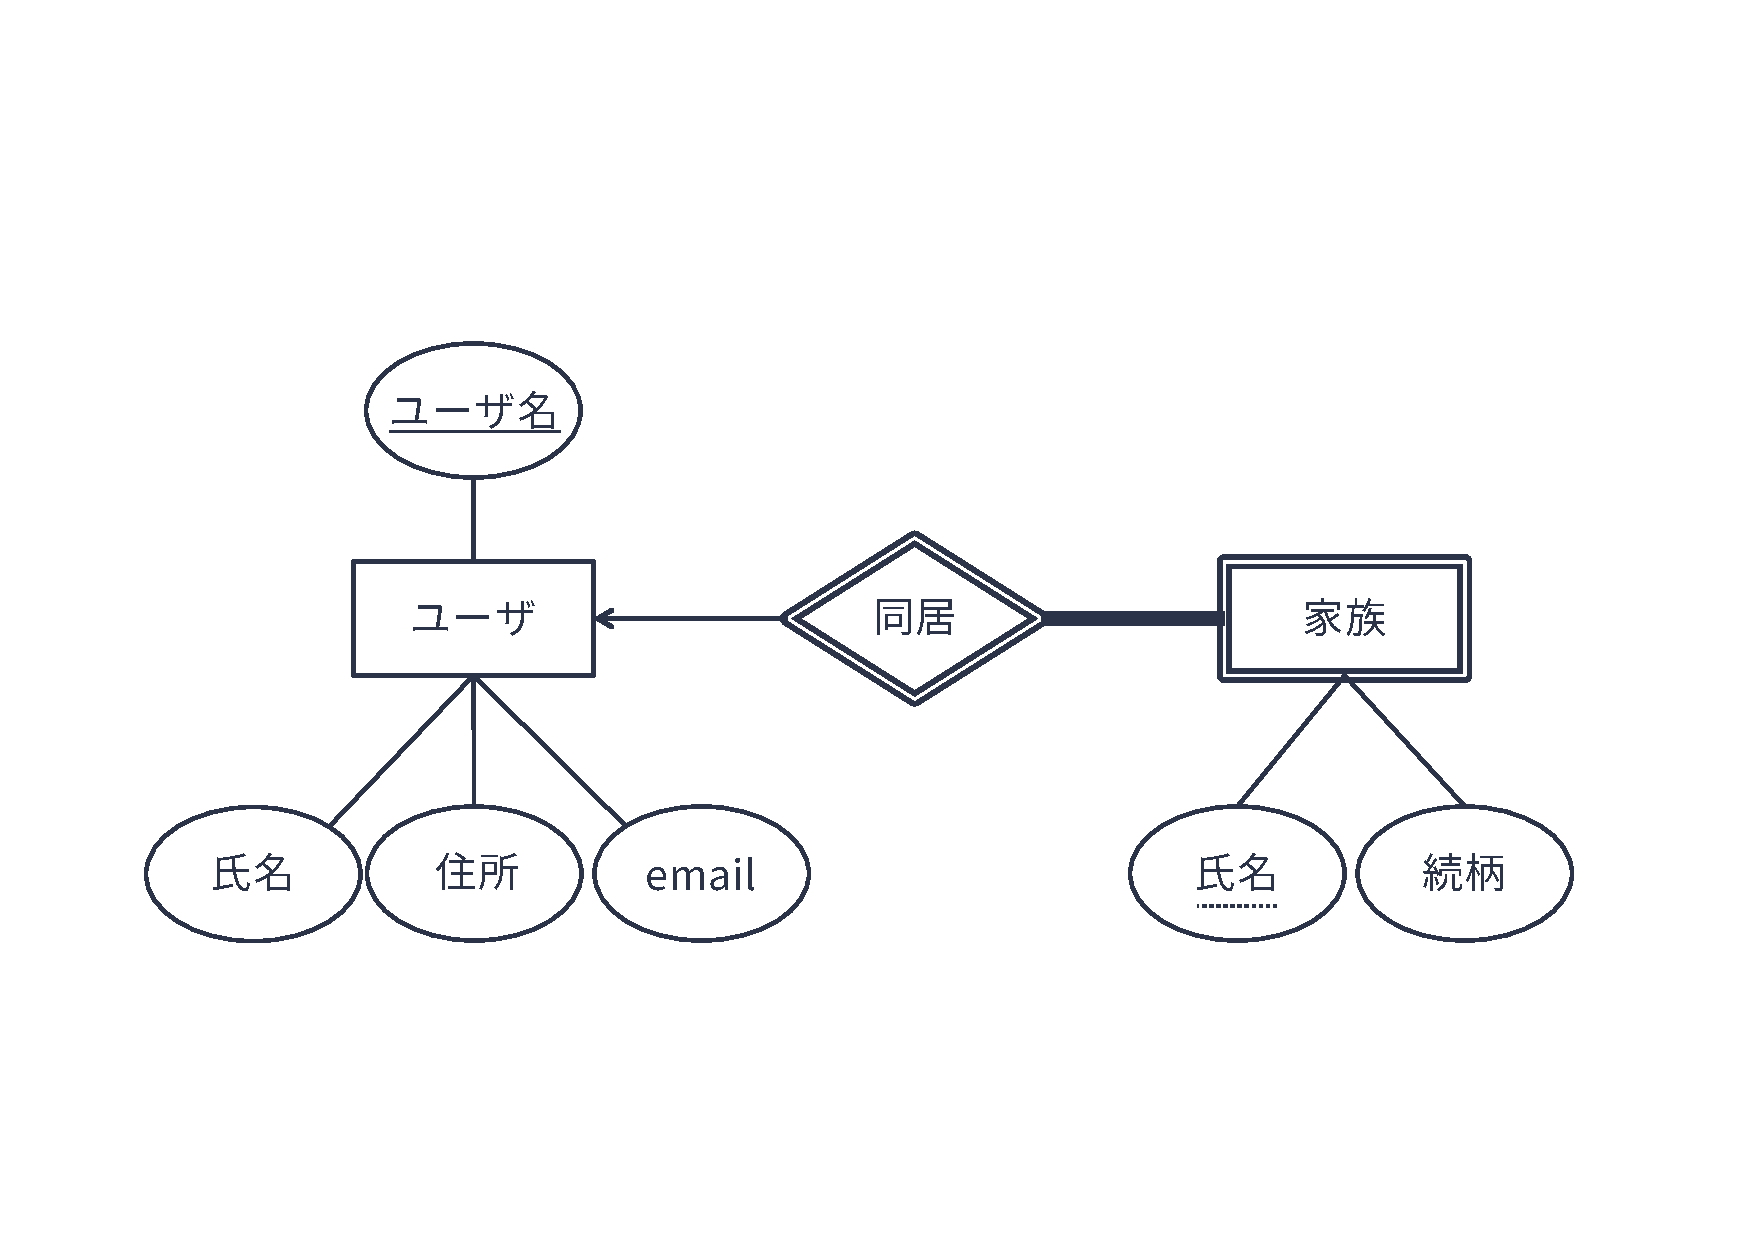
\includegraphics[width=1.0\textwidth]{figure/er-model/weak-entity.pdf}
    \caption{弱実体の例}
    \label{fig:weak_entity}
\end{figure}

図\ref{fig:weak_entity}の実体関連図を設計をすると，あるユーザを特定した際，そのユーザに関連「同居」で紐付いている実体「家族」については「氏名」によって特定が可能となります．
言い換えると，実体「ユーザ」の情報なしに「氏名」だけですべての弱実体集合「家族」に存在する，条件を満たす弱実体「家族」を特定することはできません．
これは，弱実体「家族」は自身がもつ属性だけでは主キーを構成できないことを意味します．


\begin{notebox}{弱実体はなぜ「弱」いのか？}
図\ref{fig:weak_entity}の実体関連図において，実体「家族」が弱実体としました．
読者によっては，実体「家族」にも主キーを持たせて，所有実体「ユーザ」の主キーがなくても一意に特定できるようにすればよいのでは，と考えた方がいるかもしれません．
そのようにすることも理論的にも運用上も可能です．
しかし，「家族」をあえて弱実体にしているのは，対象としているショッピングサイトの運用指針にも関係しています．

例に挙げたショッピングサイトにおいては，あくまでユーザIDをもつ「ユーザ」が販売活動の中心となっています．
あるユーザの「家族」に商品を送るというのは，その家族がユーザのIDを借りて商品を買っていると見なせます．
これは，ユーザIDを持つユーザが家族にいなければ，商品を送ってもらえない（買えない）ことを意味します．
つまり，弱実体「家族」は所有実体「ユーザ」が存在しなければ存在できない「弱い」存在であり，ある「ユーザ」が削除されるとそれと紐付いている「家族」も同時に抹消されてしまいます．

あえて「家族」を弱実体にすることは，データベースに対して「（アカウントを持つ）ユーザの存在なしにその家族の存在は認めない」というデータベース設計者の強い意図の表れと言えます．
\end{notebox}


\begin{tipbox}{弱実体にすべきか否か}
弱実体の概念は初学者には非常に難しいため，実体関連モデルの設計において弱実体を用いるべきか，迷うシーンが出てくると思います．
結論からいえば，弱実体を用いるべきかどうかは理論的に正解があるわけではなく，データベース上で対象をどう定義し，扱いたいかという設計方針によって決まります．

弱実体を用いるべきかの判断基準としては，いくつかのポイントがあります．
1つは，対象が主キーを持たせることができそうか，関連する（所有）実体の存在なしに特定できるように設計できそうかという点です．
例えば，図書館における図書の管理について考えてみましょう．
図書館は同じ書籍を複数冊所蔵して，それらを図書として貸し出せるようにしていることが多いです．
このようなケースでは，「図書」のキーを「書籍」のISBN番号と連番の組みあわせ（連番が部分キー）で表現すれば，「書籍」を所有実体，「図書」を弱実体として設計することができます．
一方，「図書」1冊1冊に図書ID（図書館専用のバーコード番号のようなもの）という一意に識別可能な値を割り振れば，理論上は「図書」を通常の実体として扱えます．
ISBN番号が何であろうと，図書館が保有しているある図書を特定できるからです．

2つ目のポイントは，運用上のメリットです．
1つ目のポイントで説明したように，ケースによっては通常の実体でも弱実体でもどちらでも設計することが可能なケースがあります．
弱実体ではなく通常の実体として扱った方が運用上のメリットがあるケースとしては，例えば，図書館の例ですと，ISBN番号が割り振られていない古い書籍を管理したい場合などが考えられます．

あえて弱実体を用いたほうが良さそうなケースとしては，弱実体として扱うべきか迷っている対象が\strong{所有実体の属性のような存在}である場合です．
例えば，先のショッピングサイトの例における「ユーザ」と「家族」の関係であったり，ショッピングサイトにおける「注文」とその「明細」の関係などが挙げられます．
どちらの例も，弱実体は所有実体の「属性」的な扱いであり，所有実体がなければ弱実体だけを管理する意味がないと考えられます．
\end{tipbox}


\section{汎化・継承}
素朴な実体関連モデルを拡張するアイデアが提案されています．
そのうちのひとつが，\strong{汎化・継承}の概念です\cite{Bancilhon1992}．

実世界を実体関連モデルで表現する際，実体集合間にある種の包含関係（階層関係）が想定される場合があります．
例えば，実体型「大学構成員」「学生」「教員」を考えてみましょう．
学生も教員も大学を構成するメンバーです．
そのため「大学構成員」と「学生」「教員」は包含関係にあると見なせます．

今，ある大学のデータ管理者は，大学構成員の情報を管理する上で，
\begin{itemize}
\item 学生には「大学ID」「氏名」「生年月日」「性別」「所属」と「入学年」
\item 教員には「大学ID」「氏名」「生年月日」「性別」「所属」と「研究者ID」「職階」
\end{itemize}
の情報を持たせたいと考えているとしましょう．
実体関連モデルで実体型「学生」「教員」を定義するには，どうしたらよいでしょうか．

ここで，あらかじめ「大学ID」「氏名」「生年月日」「性別」「所属」を属性とする実体型「大学構成員」が定義されているとしましょう．
このとき，
\begin{quotation}
実体型「学生」は属性「大学ID」「氏名」「生年月日」「性別」「所属」「入学年」を持つ実体型である
\end{quotation}
と定義するよりも，
\begin{quotation}
実体型「学生」は実体型「大学構成員」に属性「入学年」を加えた実体型である
\end{quotation}
と定義したほうが無駄が少ないですし，自然でもあります．
実体型「教員」の定義においても同様のことが言えます．
このように定義しておけば，仮に実体型「学生」と「教員」のそれぞれに「メールアドレス」という属性を持たせたいときも，実体型「大学構成員」に「メールアドレス」という属性を加えるだけで済みます．

このように，実体型$E_1$が持つすべての属性を持つと考え，新たな実体型$E_2$を定義するとき，$E_2$は$E_1$を\strong{継承（inherit）}したといいます（「$E_1$は$E2$を\strong{汎化（generalize）}した実体型である」と称することもあります）．
継承を用いて実体型を表現したとき，その実体集合（下位の集合）は継承元（上位）の実体集合にすべて包含されることになります．

実体関連図において，継承元となる上位の実体型と継承先となる下位の実体型の間には，汎化・継承関係があることを示す「isa」と記した三角の特別な関連記号を置きます．
例えば，先の実体型「大学構成員」「学生」「教員」を汎化・継承の概念を使って実体関連図を書くと，図\ref{fig:inheritance}のように表現できます．
\figure[tb]
    \centering
    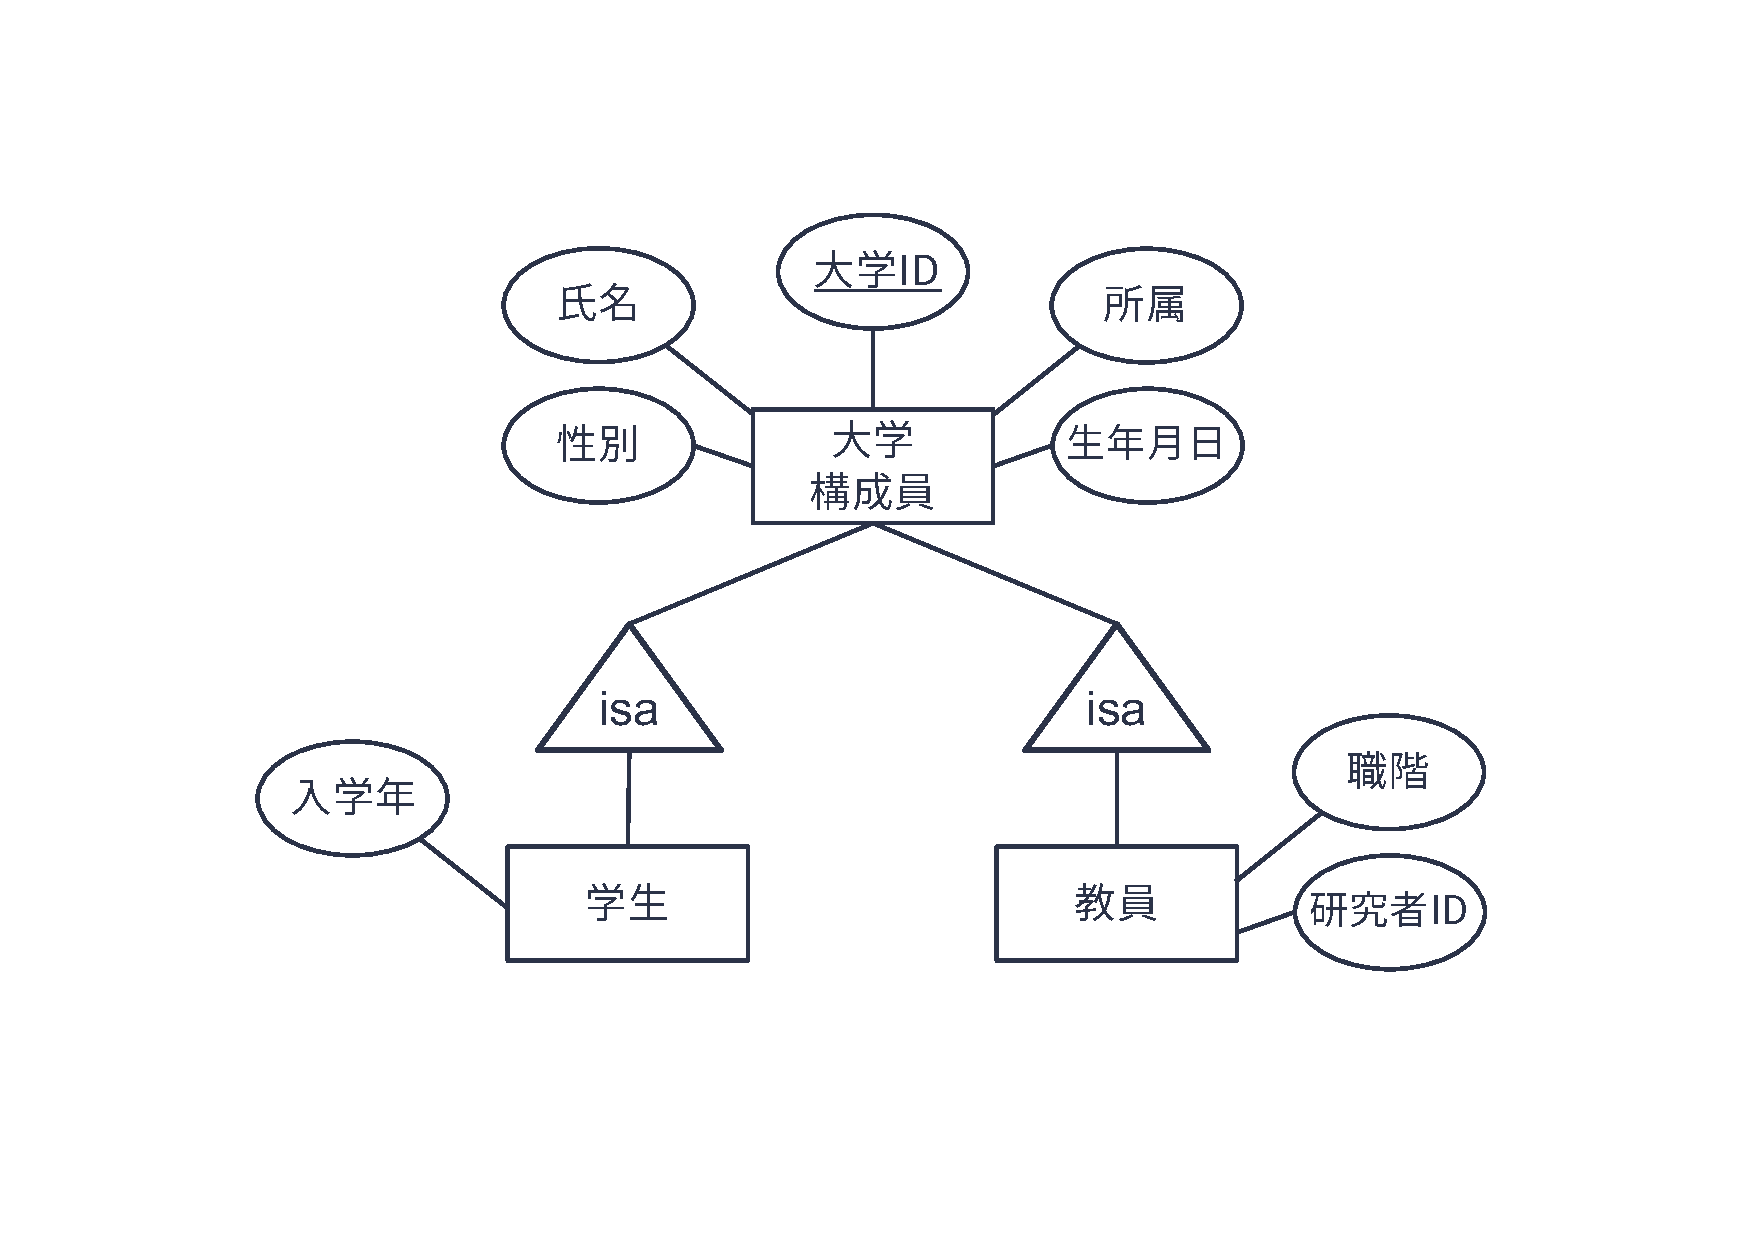
\includegraphics[width=0.8\textwidth]{figure/er-model/inheritance.pdf}
    \caption{汎化・継承の例}
    \label{fig:inheritance}
\endfigure


\section{n項関連}
これまでの説明で扱ってきた関連型は，2つの実体型とのつながりを表現したもの（2項関連）に限定されていましたが，3つ以上の実体型とつながりがあっても問題ありません．
むしろ，現実世界の状況を表現するために，3つ以上の実体型をつなぐ関連が必要になることがしばしばあります．
n個の実体型をつなぐ関連を\strong{n項関連（n-ary relationship）}と呼びます．
2項関連と同様に，n項関連においても参加制約や多重度制約を考えることができます．

\figure[htb]
    \centering
    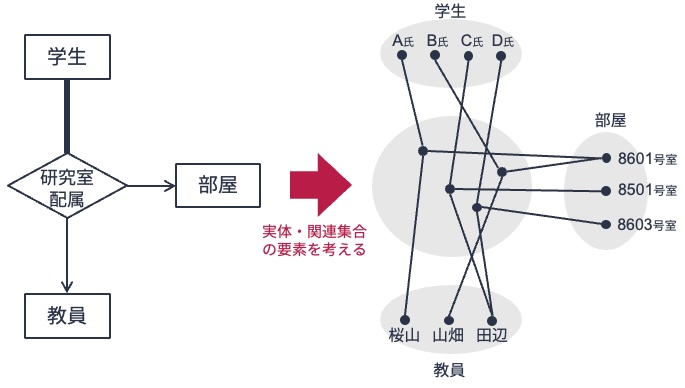
\includegraphics[width=1.0\textwidth]{figure/er-model/3-ary-relationship1.jpg}
    \caption{3項関連の例}
    \label{fig:3-aryrelationship1}
\endfigure
図\ref{fig:3-aryrelationship1}は，学生がどこの教室でどの教員の指導をうけるかを実体関連図で表現した図（左）および各実体集合，関連集合の要素を示した図（右）です．
図\ref{fig:3-aryrelationship1}では，関連型「研究室配属」は実体型「学生」「部屋」「教員」の3項関連となっています．
また，図中の実体関連図が示しているように，関連型「研究室配属」において，
\begin{itemize}
\item 「学生」と「教員」は多対1の関連
\item 「学生」と「部屋」は多対1の関連
\end{itemize}
となっています．
これは，学生の指導教員は必ず1名であり，学生に割り当てられる部屋割も必ず1つに決まる，ということを意味します．．

\figure[htb]
    \centering
    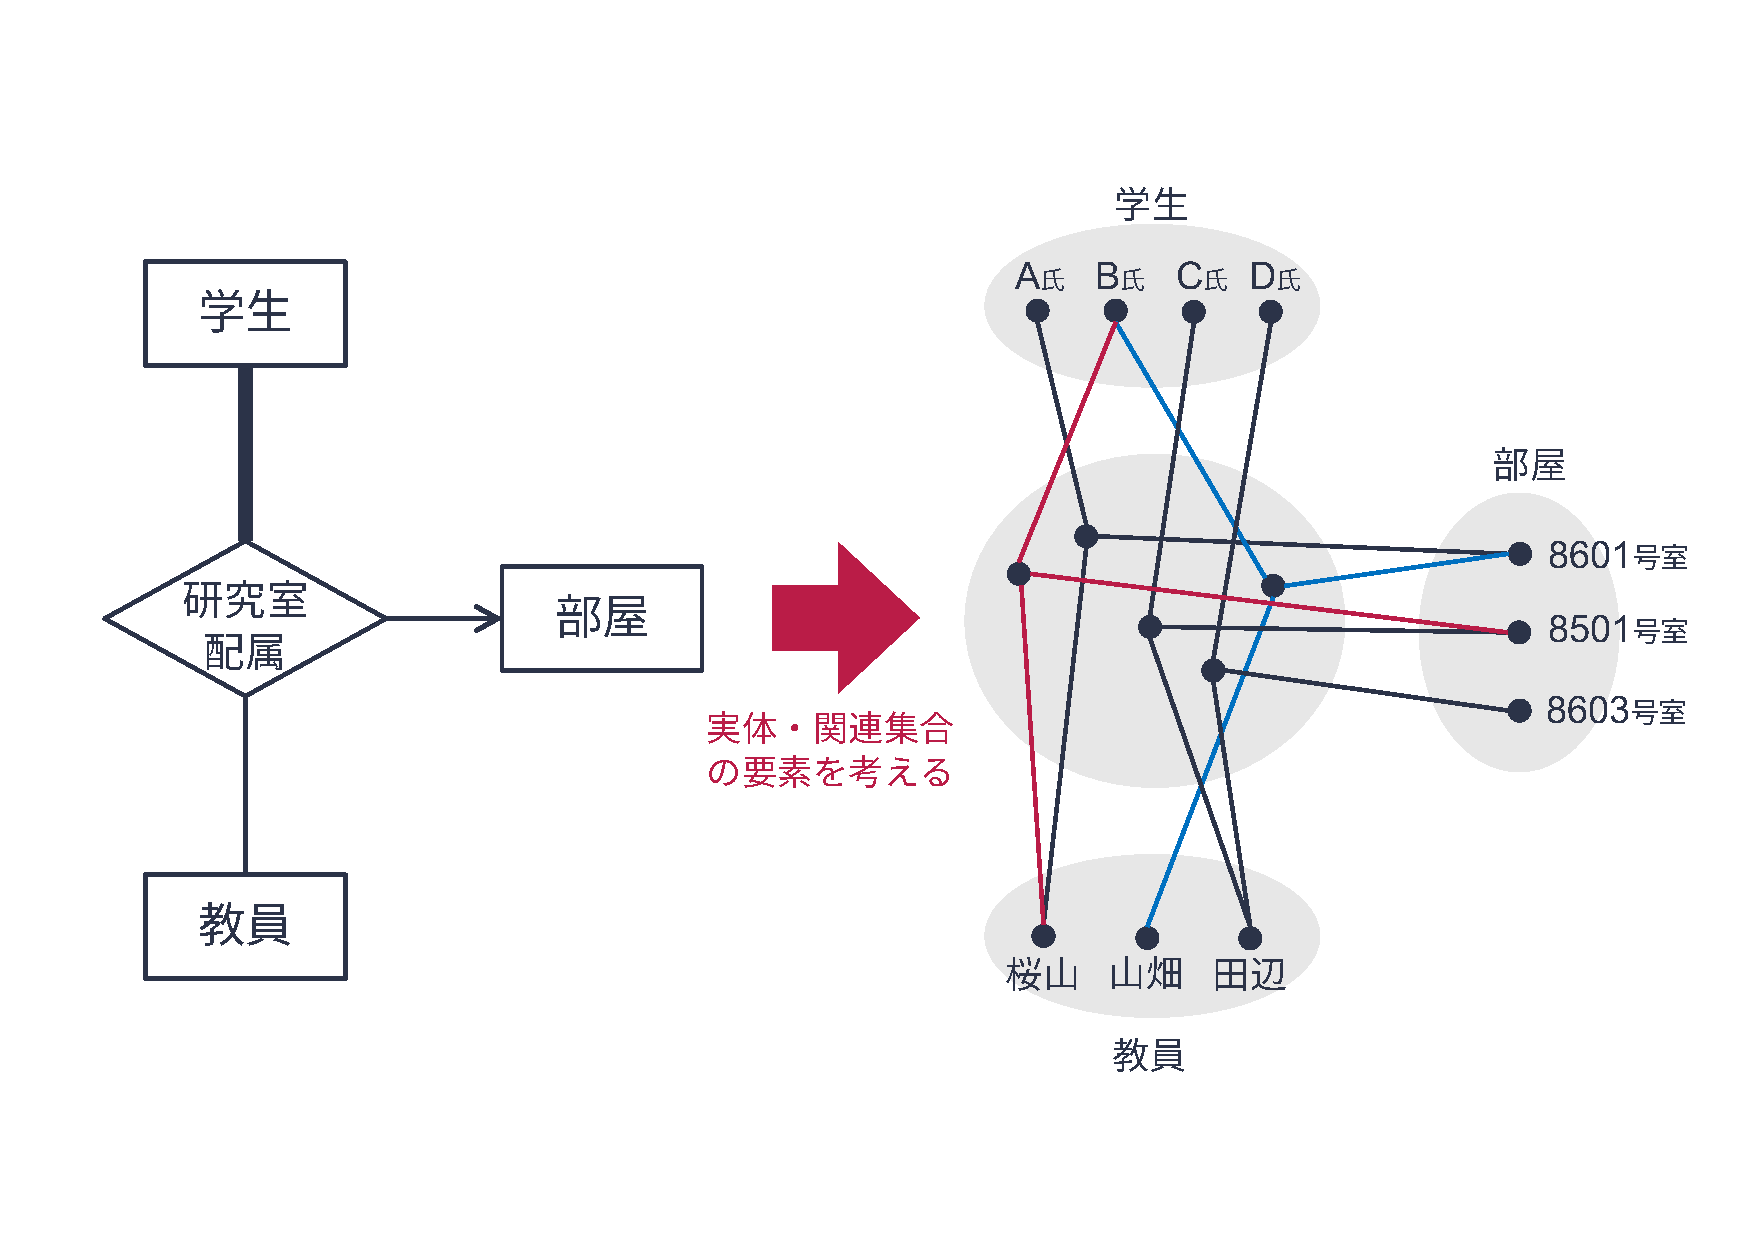
\includegraphics[width=1.0\textwidth]{figure/er-model/3-ary-relationship2.pdf}
    \caption{3項関連の例2}
    \label{fig:3-ary-relationship2}
\endfigure
一方，図\ref{fig:3-ary-relationship2}は，先ほど同様，学生がどこの教室でどの教員の指導をうけるかを表した実体関連図および各実体集合，関連集合の要素を示した図ではありますが，実体関連図で表現されている内容が微妙に異なります．
図\ref{fig:3-ary-relationship2}の実体関連図においては，
\begin{itemize}
\item 「学生」と「教員」は多対多の関連
\item 「学生」と「部屋」は多対1の関連
\end{itemize}
となっていますが，解釈には注意が必要です．
n項関連においては，ある実体集合$E$に向かう矢印は，「関連する他のすべての実体集合から実体を1つずつ選んだとき，$E$の実体が1つに決まる」を意味すると定義されています．
これを踏まえると，図\ref{fig:3-ary-relationship2}においては，\strong{学生と教員の組みあわせ}に対応して部屋が1つに決まる，ということを意味します．
2項関係のように
\begin{itemize}
    \item 学生には複数の教員を割り当てることができる
    \item 学生に割り当てられる部屋は必ず1つである
\end{itemize}
と解釈してはいけません．
この実体関連図に対応する要素に関する図（図\ref{fig:3-ary-relationship2}の右図）を見ると，学生Bには桜山先生と山畑先生の2名の教員が指導教員として割り当てられていますが，部屋割は学生と教員の組みあわせに対して行われるため，学生Bは8501号室と8601号室の2部屋が割り当てられていることが分かります．


\section{実体関連モデルから関係スキーマへの変換}
本書で実体関連モデルを学ぶ理由は，実体関連モデルを関係データベースの設計に活用するためでした．
学習の締めくくりとして，実体関連モデルを関係スキーマに変換する方法を説明します．

実体関連モデルは概念モデルであり，そのままでは関係データベースシステム上で扱うことはできません．
そのため，論理モデルである関係データモデルに変換する必要があります．
この作業はそれほど難しいものではありません．
前節までに学習した実体関連図を用いれば，関係データモデルの構造を示す関係スキーマを\strong{機械的に}導出することができます．

以下，実体関連図のパターンに応じた関係スキーマへの変換方法を説明します．
説明には，実体関連モデルの解説で用いたオンラインショッピングの例を用います．

\subsection{変換パターン1：実体型}
実体型は
\begin{itemize}
\item 実体型名を関係スキーマの関係名
\item 実体型のキーを関係スキーマのキー
\item 実体型の属性を関係スキーマの属性
\end{itemize}
に対応させることで関係スキーマに変換できます．

図\ref{fig:erd-entity}に示した実体型「ユーザ」は以下のような関係スキーマに変換される
\begin{figure}[tb]
  \centering
  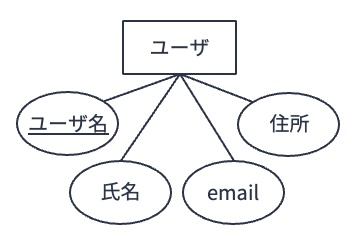
\includegraphics[width=0.6\textwidth]{figure/er-model/erd-entity.jpg}
  \caption{実体型「ユーザ」}
  \label{fig:erd-entity}
\end{figure}
\begin{equation}
  \text{ユーザ}(\underline{\text{ユーザ名}}, \text{氏名}, \text{住所}, \text{email})
\end{equation}


\subsection{変換パターン2：関連型}
関連型を関係スキーマに変換するには，基本的には
\begin{itemize}
\item 関連型名を関係スキーマの関係名
\item 関連型とつながる実体型のキーを関連型のキー
\item （あれば）関連型の属性を関係スキーマの属性
\end{itemize}
に対応させればよいです．
ただし，実体関連間の多重度によってキーの扱いが異なります．

\subsubsection{多重度が「多対多」の場合}
\begin{figure}[tb]
  \centering
  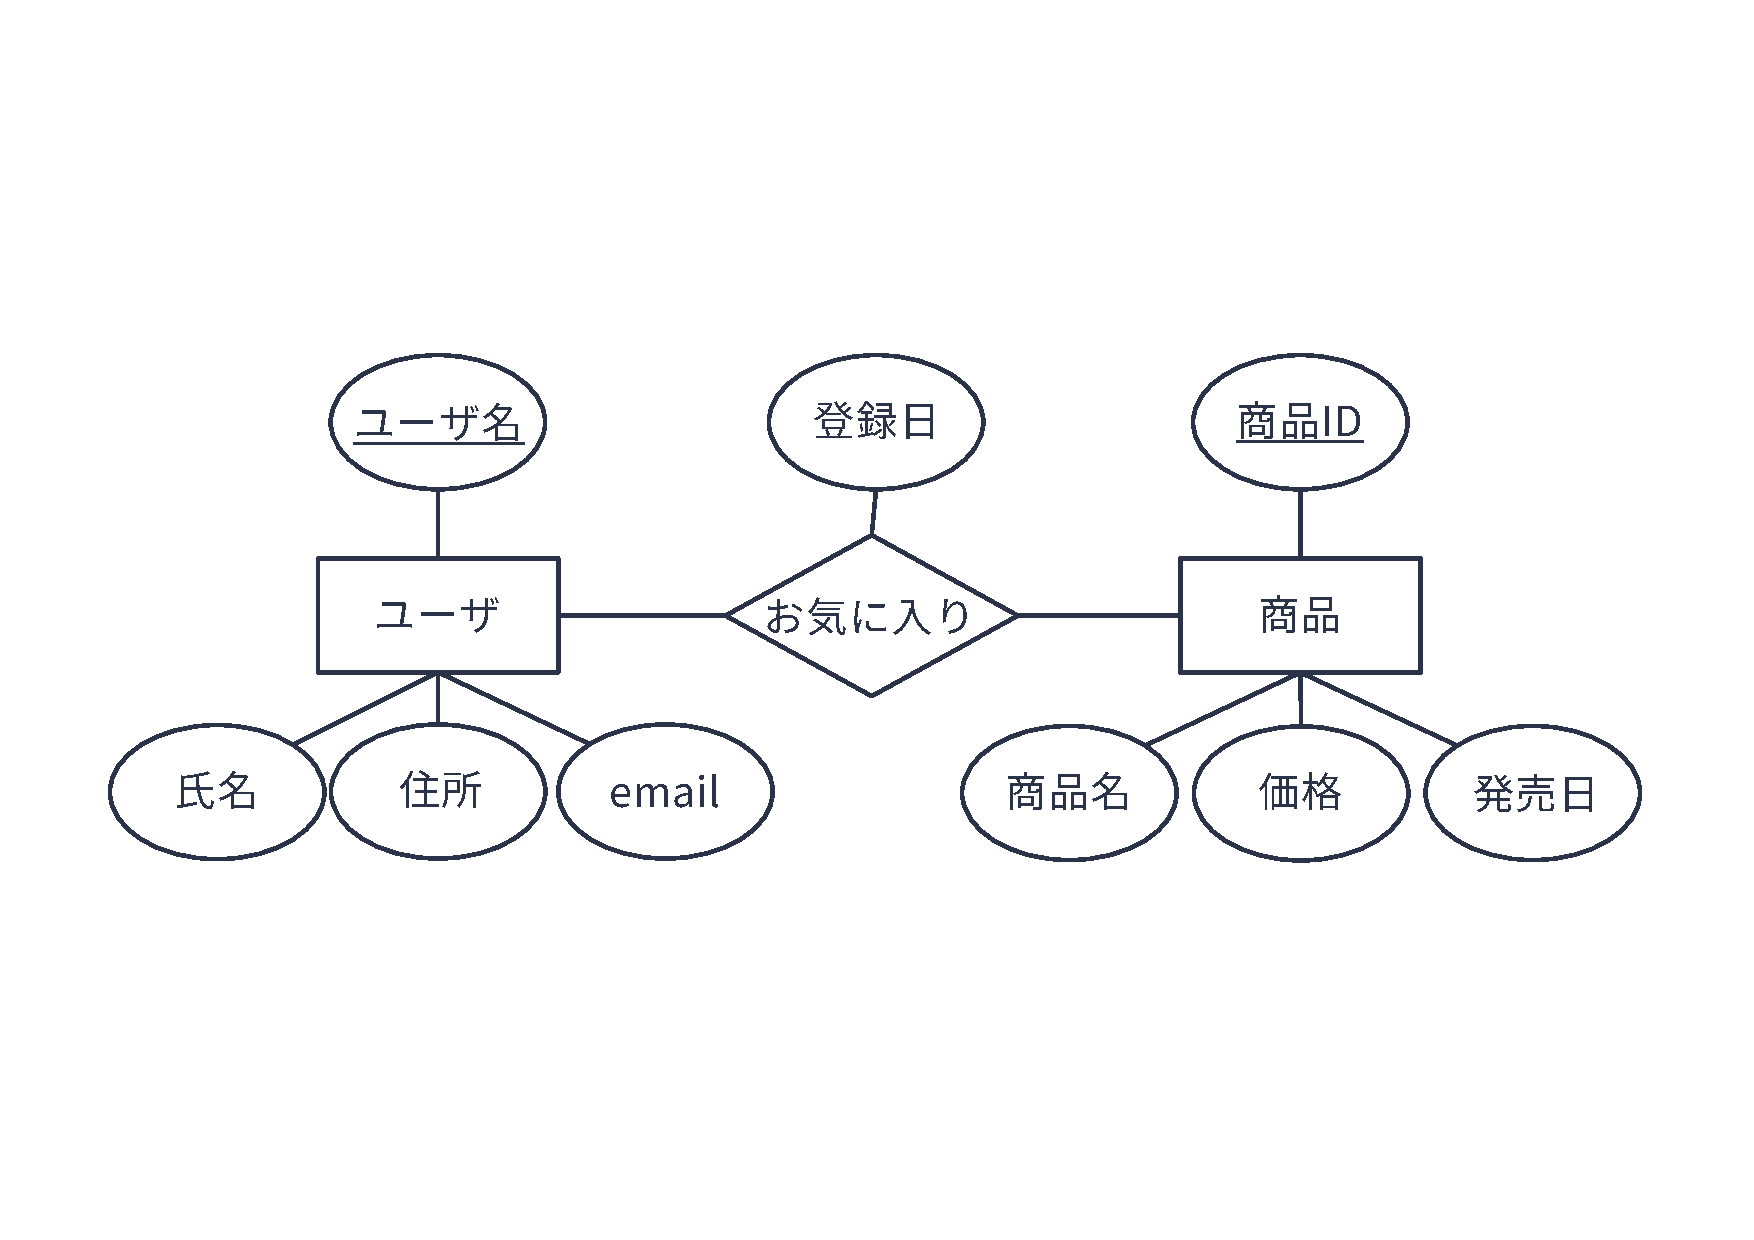
\includegraphics[width=0.9\textwidth]{figure/er-model/erd-relation1.pdf}
  \caption{多対多の関連型「お気に入り」}
  \label{fig:erd-relation1}
\end{figure}
図\ref{fig:erd-relation1}では，実体型「ユーザ」と「商品」は関連型「お気に入り」を介して多対多の関連でつながっています．

このような「多対多」の関連を関係スキーマに変換する場合は，関連を一意に識別するために，\strong{関連型につながるすべての実体型の主キーを集めたもの}を関連型の主キーとします．
図\ref{fig:erd-relation1}の場合，実体型「ユーザ」の主キーは\graybox{ユーザ名}，「商品」の主キーは\graybox{商品ID}であるため，関連型「お気に入り」の主キーは\graybox{\{ユーザ名, 商品ID\}}となります\footnote{このように属性の組みあわせによって構成された主キーは複合主キーと呼ばれます．複合主キーは理論上正しいのですが，実務では管理を容易にするためにシステムが自動的に付与する人工的な主キー「代理キー（surrogate key）」を持たせることがあります．代理キーの例としては，連番や重複しない文字列（UUID）などが挙げられます}．
結果的に，関連型「お気に入り」は以下のような関係スキーマに変換されます．
\begin{equation}
  \text{お気に入り}(\underline{\text{ユーザ名}, \text{商品ID}}, \text{登録日})
\end{equation}

ところで，関連型の関係スキーマの主キーは関連している実体型の主キーから構成されるため，対象となる関連型および実体型を変換した関係スキーマの間には参照整合制約が生じます．
つまり，関連型の主キーは，関連している（つながっている）実体型に対する外部キーとなります．
例えば，先の例の関係「お気に入り」の主キーである\graybox{ユーザ名}と\graybox{商品ID}は，関係「ユーザ」および「商品」に対する外部キーになります．
「お気に入り」の主キーである\graybox{ユーザ名}と\graybox{商品ID}の値は，必ず関係「ユーザ」の\graybox{ユーザ名}の属性値，「商品」の\graybox{商品ID}の属性値として存在している必要があります．
よって，上記関連型を関係スキーマに変換したときには，
\begin{eqnarray}
  \text{ユーザ}(\underline{\text{ユーザ名}}, \text{氏名}, \text{住所}, \text{email}) \label{eq:user}\\
  \text{商品}(\underline{\text{商品ID}}, \text{商品名}, \text{価格}, \text{発売日}) \label{eq:product}\\
  \text{お気に入り}(\underline{\text{ユーザ名}, \text{商品ID}}, \text{登録日}) \label{eq:favorite}\\
  \text{お気に入り.ユーザ名} \subseteq \text{ユーザ.ユーザ名} \label{eq:favorite-fk1}\\
  \text{お気に入り.商品ID} \subseteq \text{商品.商品ID} \label{eq:favorite-fk2}
\end{eqnarray}
が参照整合性制約を含めた関係スキーマとなります．


\subsubsection{多重度が「多対1」の場合}
\figure[tb]
  \centering
  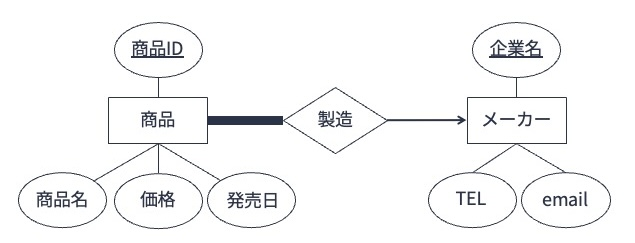
\includegraphics[width=0.9\textwidth]{figure/er-model/erd-relation2.jpg}
  \caption{多対1の関連型「製造」}
  \label{fig:erd-relation2}
\endfigure

図\ref{fig:erd-relation2}では，実体型「商品」と「メーカー」は関連型「製造」を介して多対1の関連でつながっています．
すなわち，実体集合「商品」の実体要素が決まれば，それに対応する実体集合「メーカー」の実体要素が必ず1つ特定されることになります．

このような「多対1」の関連型の場合，矢印のついていない側の実体の主キーの値が決まれば，矢印のついている側の実体が一意に特定されると同時に関連の要素も一意に特定されます．
そのため，関係スキーマに変換する場合は，\strong{関連型につながる，矢印のついていない側の実体型の主キー}を関連型の主キーとします．

図\ref{fig:erd-relation2}を関係スキーマに変換すると，以下のようになります．
関係「製造」において\graybox{企業名}が属性になりますが，主キーにはならない（含まれない）ことに注意しましょう．
\begin{eqnarray}
  \text{商品}(\underline{\text{商品ID}}, \text{商品名}, \text{価格}, \text{発売日}) \\
  \text{メーカー}(\underline{\text{企業名}}, \text{TEL}, \text{email}) \\
  \text{製造}(\underline{\text{商品ID}}, \text{企業名}) \\
  \text{製造.商品ID} \subseteq \text{商品.商品ID}\\
  \text{製造.企業名} \subseteq \text{メーカー.企業名}
\end{eqnarray}

\subsubsection{多重度が「1対1」の場合}
\figure[tb]
  \centering
  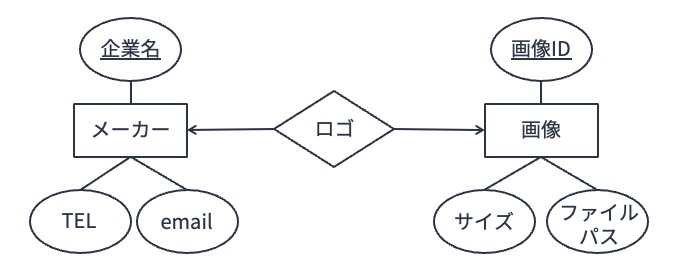
\includegraphics[width=0.9\textwidth]{figure/er-model/erd-relation3.jpg}
  \caption{1対1の関連型「ロゴ」}
  \label{fig:erd-relation3}
\endfigure
図\ref{fig:erd-relation3}では，実体型「メーカー」と「画像」は関連型「ロゴ」を介して1対1の関連でつながっています．

このような「1対1」の関連型の場合，関連している\strong{いずれか}の実体型の主キーの値が決まれば，関連の要素も一意に特定されます．
そのため，関係スキーマに変換する場合は，\strong{関連型につながる，いずれかの実体型の主キー}を関連型の主キーとします．

図\ref{fig:erd-relation3}を関係スキーマに変換すると，以下のようになります．
関係「ロゴ」においては，\graybox{画像ID}が属性になるが主キーにならない（含まれない）ことに注意しましょう．
\begin{eqnarray}
  \text{メーカー}(\underline{\text{企業名}}, \text{TEL}, \text{email}) \\
  \text{画像}(\underline{\text{画像ID}}, \text{ファイル名}, \text{サイズ}) \\
  \text{ロゴ}(\underline{\text{企業名}}, \text{画像ID}) \\
  \text{ロゴ.企業名} \subseteq \text{メーカー.企業名}\\
  \text{ロゴ.画像ID} \subseteq \text{画像.画像ID}
\end{eqnarray}


\subsection{変換パターン3：汎化・継承}
実体型$E_1$を継承した実体型$E_2$を関係スキーマに変換するには，実体型と同じ変換方法を用いればよいです．
すなわち
\begin{itemize}
\item 継承先の実体型名を関係スキーマの関係名
\item 継承元の実体型のキーを関係スキーマのキー
\item 継承先の実体型の属性を関係スキーマの属性
\end{itemize}
に対応させればよいです．
継承先の実体型の主キーは継承元の実体型の主キーとすることに注意しましょう．

\figure[tb]
  \centering
  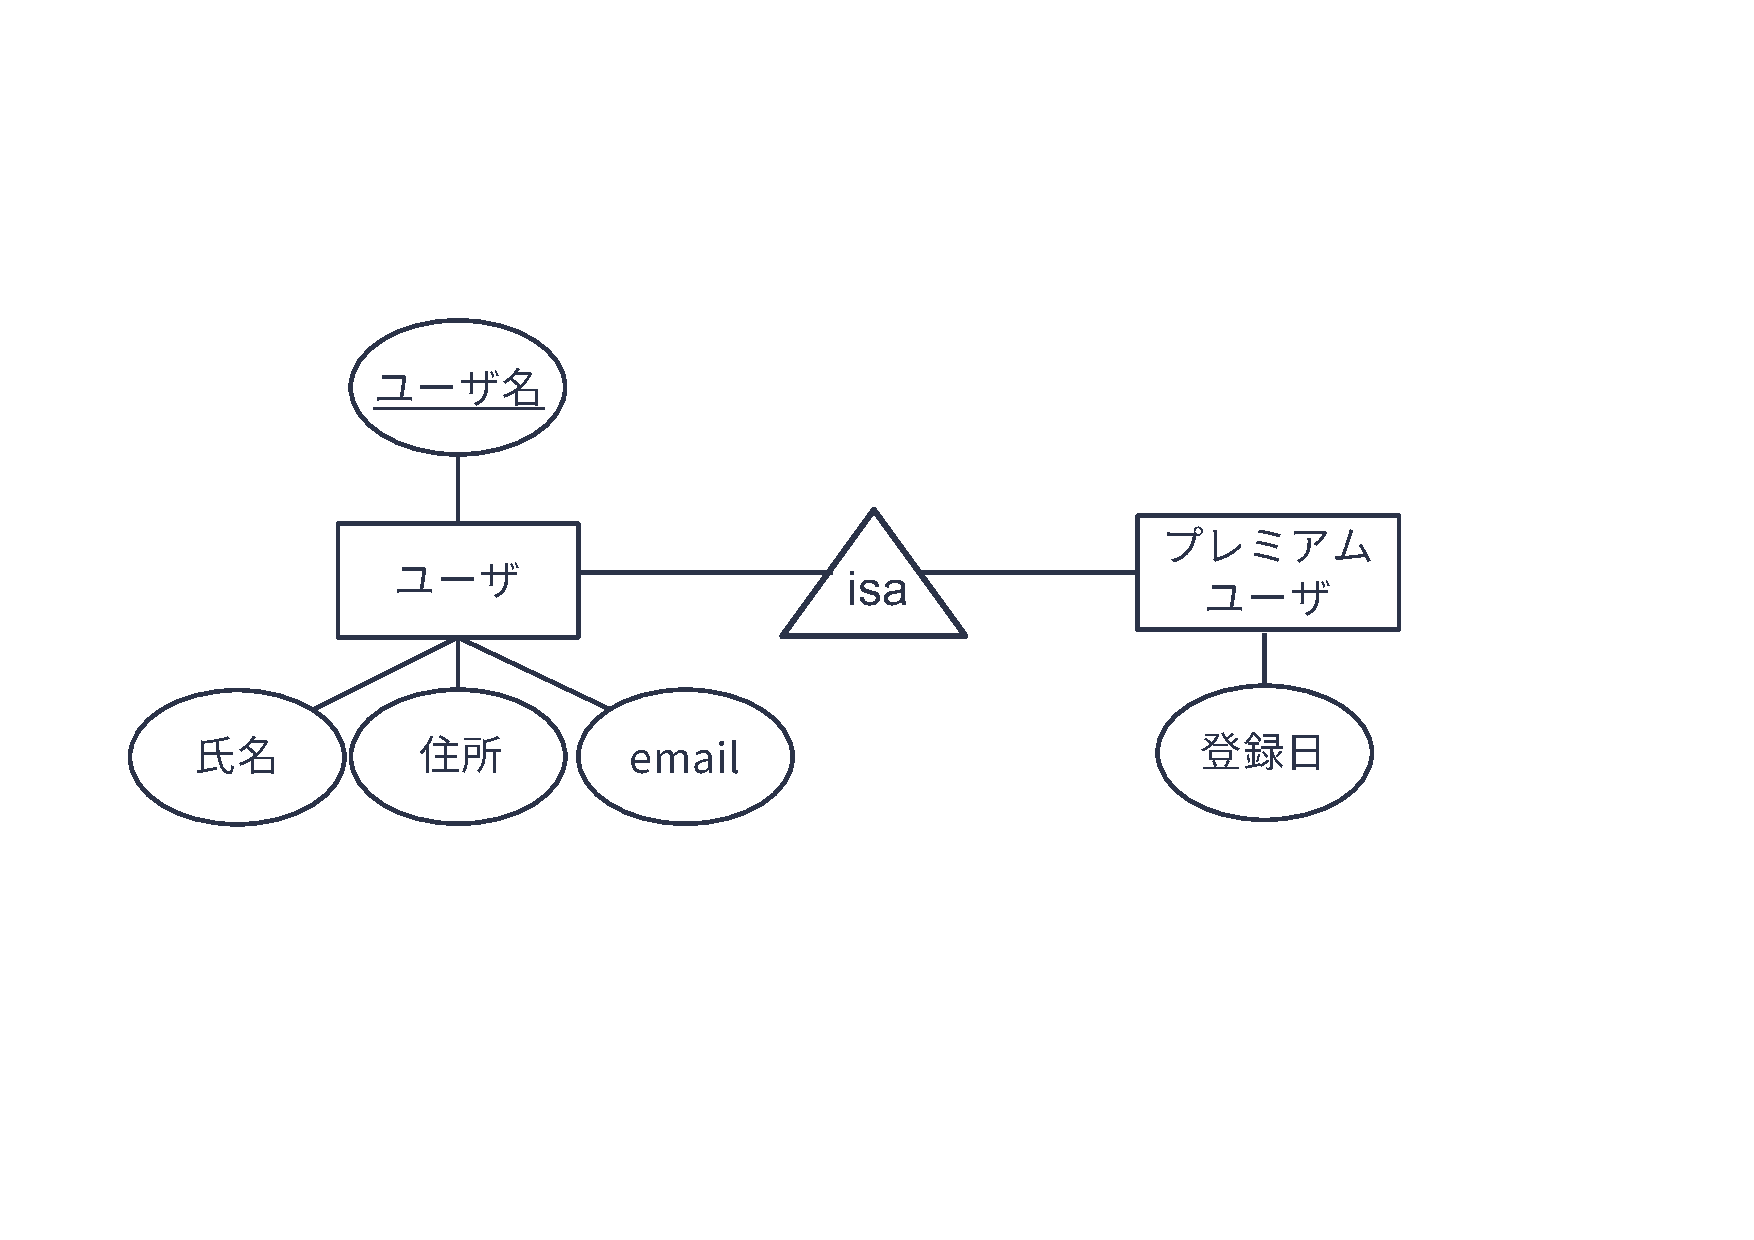
\includegraphics[width=0.8\textwidth]{figure/er-model/erd-inheritance.pdf}
  \caption{実体型「ユーザ」を継承した実体型「プレミアムユーザ」}
  \label{fig:erd-inheritance}
\endfigure
図\ref{fig:erd-inheritance}に示した実体型「プレミアムユーザ」は，以下のような関係スキーマに変換されます．
\begin{equation}
  \text{プレミアムユーザ}(\underline{\text{ユーザ名}}, \text{登録日})
\end{equation}


\subsection{変換パターン4：弱実体型と弱関連型}
\figure[tb]
  \centering
  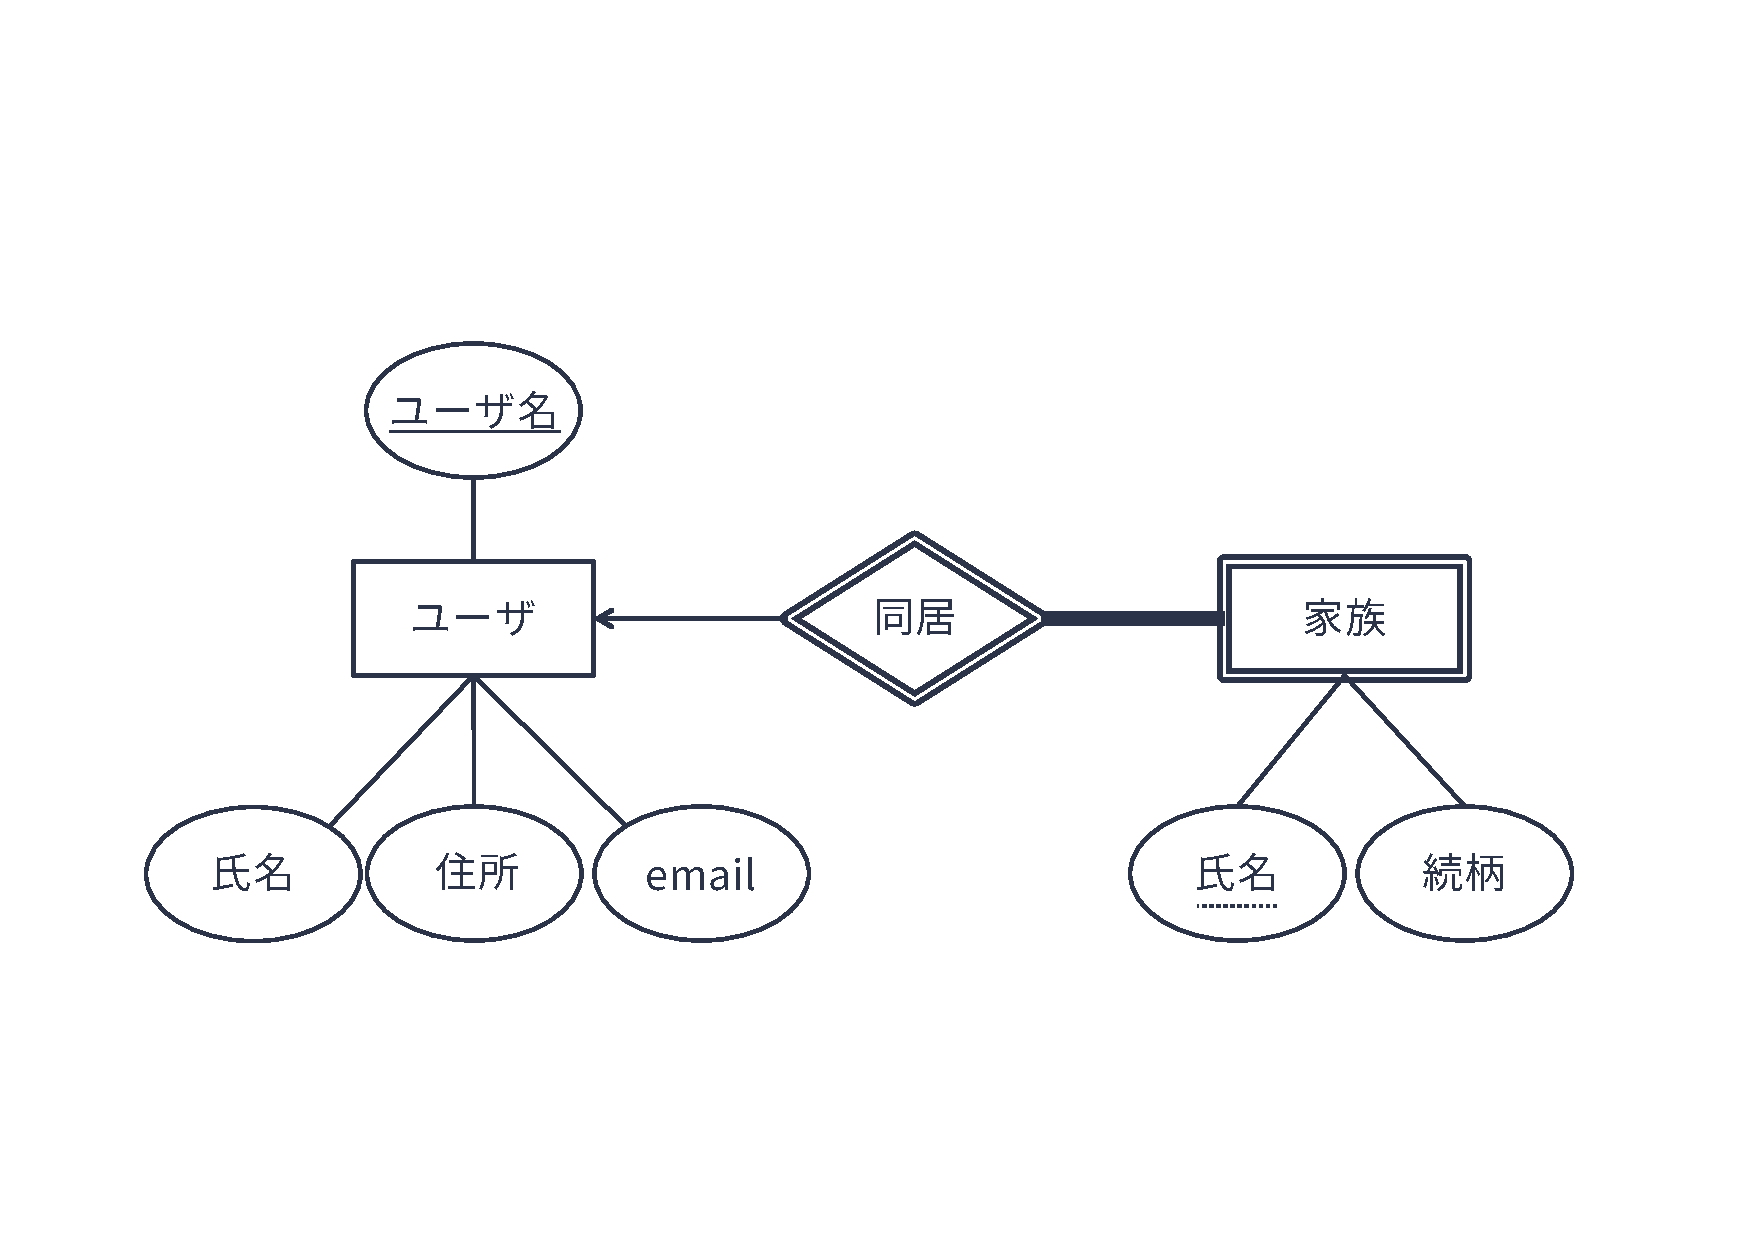
\includegraphics[width=0.9\textwidth]{figure/er-model/weak-entity.pdf}
  \caption{弱実体型「家族」と弱関連型「所属」}
  \label{fig:weak-entity-relation}
\endfigure
図\ref{fig:weak-entity-relation}のような弱実体・弱関連の関係スキーマへの変換はややトリッキーです．
弱実体は自らの属性だけでは一意に特定できないため，弱関連型を通じてつながる（所有）実体型の主キーと自らの属性（部分キー）をセットにして主キーとする必要がありました．
このことを踏まえて，弱実体型は以下のように関係スキーマに変換します．
\begin{itemize}
\item 弱実体型の名前を関係スキーマの関係名にする
\item 弱実体型の部分キーおよび弱実体型とつながる（所有）実体型の主キーをセットにしたものを関係の主キーとする
\item 弱実体型の属性を関係スキーマの属性とする
\end{itemize}

図\ref{fig:weak-entity-relation}の弱実体型「家族」は以下のような関係スキーマに変換されます．
\begin{equation}
  \text{家族}(\underline{\text{ユーザ名}, \text{氏名}}, \text{続柄})
\end{equation}

なお，弱実体型の主キーを構成する要素のうち，部分キーでない方は別の実体型の主キーを借りているため，参照整合性制約が生じます．
先の例の弱実体型「家族」であれば，\graybox{ユーザ名}が外部キーに相当します．
そのため，以下のような参照整合性制約を関係スキーマに加える必要があります．
\begin{equation}
  \text{家族.ユーザ名} \subseteq \text{ユーザ.ユーザ名}
\end{equation}

弱関連型は
\begin{itemize}
\item 弱関連型名を関係スキーマの関係名
\item 自らの部分キーと弱関連型でつながる（所有）実体型の主キーのセットを関係スキーマの主キー
\item 弱関連型の属性を関係スキーマの属性
\end{itemize}
に対応させることで関係スキーマに変換します．

図\ref{fig:weak-entity-relation}の弱関連型「同居」は，以下のような関係スキーマに変換されます．
\begin{eqnarray}
  \text{同居}(\underline{\text{ユーザ名}, \text{氏名}}) \\
  \text{同居.ユーザ名} \subseteq \text{ユーザ.ユーザ名} \\
  \text{同居.氏名} \subseteq \text{家族.氏名} \\
\end{eqnarray}

ところで，弱実体型「家族」は，弱関連型「同居」に対する参加制約が全体的です．
また，弱実体型「家族」に対応する関係スキーマ「家族」の属性は弱関連型「同居」に対応する関係スキーマ「同居」の属性を包含しています．
これは，関係「家族」があれば関係「同居」は把握でき，関係「同居」は不要であることを意味します．
結果的に，関係「同居」は削除できます．


\section{レコードを追加，修正，削除するためのSQL}
関係スキーマが定義できれば，いよいよ関係データベースにレコードの追加，修正，削除が可能となります．
レコードの追加，修正，削除には，\ref{chap:sql-part1}で紹介した関係データベースの問い合わせ言語であるSQLを用います．
以下では，SQLを用いてレコードの追加，修正，削除を行うための基本的な方法を説明します．

\subsection{テーブルの定義}
レコードを追加するには，まず関係データベース内にレコードを追加するテーブルを定義する必要があります．
これまでに説明してきた関係スキーマは，このテーブル定義に活かされます．

SQLでテーブルの定義を行うには，\graybox{CREATE TABLE}文を用います．
\graybox{CREATE TABLE}文の構文はコード\ref{code:create-table-structure}のようになっています．
ここで，テーブル名は関係スキーマにおける関係名，列名は属性名に対応します．
主キーや外部キーは，それぞれ関係スキーマで指定している主キー制約，参照整合性制約に対応します．
\begin{figure}[h]
    \begin{minted}[gobble=1,
        bgcolor=background,
        fontsize=\small,
        linenos=false,
        xleftmargin=0em]{sql}

    CREATE TABLE テーブル名 (
        列名1 データ型 [制約],
        列名2 データ型 [制約],
        ...
        [主キー]
        [外部キー]
    );
    \end{minted}
    \captionsetup{name=コード}
    \caption{CREATE TABLE文の構文．[ ]は省略可能な要素を示す．}
    \label{code:create-table-structure}
\end{figure}

データ型は\ref{chap:relational-data-model}で説明したドメイン制約に対応するものです．
SQLでは整数や文字列など，単純なドメイン制約を指定するデータ型が用意されています．
代表的なデータ型は以下の通りです：
\begin{itemize}
\item \graybox{INT}：整数型
\item \graybox{VARCHAR(n)}：（最大$n$文字の長さの）文字列型
\item \graybox{FLOAT}：浮動小数点数型
\item \graybox{BOOLEAN}：真偽値型
\item \graybox{DATETIME}：時刻を併せ持つ日付型
\end{itemize}
ドメイン制約では属性値は「整数でなければならない」といった単純な制約だけでなく，
\begin{itemize}
\item 0以上10000以下の整数でなければならない
\item xxx，yyy，zzzのいずれかでなければならない
\item @xxxx.comの形式の文字列で終わらなければならない
\end{itemize}
といった複雑な制約が必要になることもあります．
このような複雑な制約を\graybox{CREATE TABLE}文で指定するには，\graybox{CREATE DOMAIN}文でドメインを定義し，そのドメインをテーブル定義のデータ型に指定する方法があります．
これについては本書のレベルを超える内容になるため，ここでの説明は割愛します．

\graybox{CREATE TABLE}文における列名の「制約」には，その列に対する様々な制約を指定することができます．
代表的な制約は以下の通りです：
\begin{itemize}
\item \graybox{NOT NULL}：NULL値を許さない制約
\item \graybox{UNIQUE}：重複する値を許さない制約
\item \graybox{PRIMARY KEY}：主キー制約
\item \graybox{REFERENCES}：参照整合性制約（外部キーの指定）
\end{itemize}

例えば，式\ref{eq:user}で定義した関係スキーマ「ユーザ」，式\ref{eq:product}で定義した関係スキーマ「商品」を用いてテーブル定義するには，コード\ref{code:create-table}のような\graybox{CREATE TABLE}文を用います．
\begin{figure}[h]
    \begin{minted}[gobble=1,
        bgcolor=background,
        fontsize=\small,
        linenos=false,
        xleftmargin=0em]{sql}

    CREATE TABLE ユーザ (
        ユーザ名 VARCHAR(100) PRIMARY KEY, --- コメント: 文字列長は最大100文字とする
        氏名 VARCHAR(100) NOT NULL,
        住所 VARCHAR(100) NOT NULL,
        email VARCHAR(100) NOT NULL
    );

    CREATE TABLE 商品 (
        商品ID VARCHAR(100) PRIMARY KEY,
        商品名 VARCHAR(100) NOT NULL,
        価格 INT NOT NULL,
        発売日 DATETIME NOT NULL
    );

    \end{minted}
    \captionsetup{name=コード}
    \caption{テーブル「ユーザ」「商品」を定義するCREATE TABLE文の例．}
    \label{code:create-table}
\end{figure}

主キーおよび外部キーの指定は，列定義の中で指定する方法と，テーブル全体の制約として指定する方法があります．
主キーが複数の列の組みあわせで構成されるなど，複雑な主キーや外部キーを指定する場合は，テーブル全体の制約として指定する方法が適しています．
コード\ref{code:create-table2}は，式\ref{eq:favorite}-\ref{eq:favorite-fk2}で定義した関係スキーマ「お気に入り」をテーブル定義するための\graybox{CREATE TABLE}文の例です．
\begin{figure}[h]
    \begin{minted}[gobble=1,
        bgcolor=background,
        fontsize=\small,
        linenos=false,
        xleftmargin=0em]{sql}

    CREATE TABLE お気に入り (
        ユーザ名 VARCHAR(100) NOT NULL,
        商品ID VARCHAR(100) NOT NULL,
        登録日 DATETIME NOT NULL,
        --- コメント: 主キーはユーザ名と商品IDの組みあわせ
        PRIMARY KEY (ユーザ名, 商品ID),
        --- テーブル「お気に入り」の「ユーザ名」はテーブル「ユーザ」の「ユーザ名」に対する外部キーとなる
        FOREIGN KEY (ユーザ名) REFERENCES ユーザ(ユーザ名)
    );

    \end{minted}
    \captionsetup{name=コード}
    \caption{テーブル「お気に入り」を定義するSQL文の例．}
    \label{code:create-table2}
\end{figure}


\subsection{レコードの追加}
テーブルにレコードを追加するには，\graybox{INSERT}文を用います．
\graybox{INSERT}文の構文はコード\ref{code:insert-into-structure}のようになっています．
\begin{figure}[h]
    \begin{minted}[gobble=1,
        bgcolor=background,
        fontsize=\small,
        linenos=false,
        xleftmargin=0em]{sql}

    INSERT INTO
        テーブル名 (列名1, 列名2, ...)
    VALUES
        (レコード1件目の属性1の値, 属性2の値, ...),
        (レコード1件目の属性2の値, 属性2の値, ...)
        ... ;
    \end{minted}
    \captionsetup{name=コード}
    \caption{INSERT文の構文}
    \label{code:insert-into-structure}
\end{figure}

コード\ref{code:insert-into-example}は，先ほど取り上げた\graybox{商品}テーブルに3件のレコードを追加するためのSQL文の例です．
\begin{figure}[h]
    \begin{minted}[gobble=1,
        bgcolor=background,
        fontsize=\small,
        linenos=false,
        xleftmargin=0em]{sql}

    INSERT INTO
        商品 (商品ID, 商品名, 価格, 発売日)
    VALUES
        ('P001', 'はーいお茶', 130, '1989-02-01 09:00:00'),
        ('P002', 'きのこの里', 230, '2019-08-06 10:00:00'),
        ('P003', 'のど飴', 170, '2016-02-16 14:30:00');

    \end{minted}
    \captionsetup{name=コード}
    \caption{テーブル「商品」にレコードを追加するSQL文の例}
    \label{code:insert-into-example}
\end{figure}

\subsection{レコードの削除}
テーブル中のレコードを削除するには，\graybox{DELETE}文を用います．
\graybox{DELETE}文の構文はコード\ref{code:delete-structure}のようになっています．
\begin{figure}[h]
    \begin{minted}[gobble=1,
        bgcolor=background,
        fontsize=\small,
        linenos=false,
        xleftmargin=0em]{sql}

    DELETE FROM
        テーブル名
    WHERE
        条件 ;

    \end{minted}
    \captionsetup{name=コード}
    \caption{DELETE文の構文}
    \label{code:delete-structure}
\end{figure}

コード\ref{code:delete-example}は，先ほど取り上げた\graybox{商品}テーブルから特定のレコードを削除するためのSQL文の例です．
\begin{figure}[h]
    \begin{minted}[gobble=1,
        bgcolor=background,
        fontsize=\small,
        linenos=false,
        xleftmargin=0em]{sql}

    DELETE FROM
        商品
    WHERE
        価格 <= 100;

    \end{minted}
    \captionsetup{name=コード}
    \caption{テーブル「商品」から価格が100円以下のレコードを削除するSQL文の例}
    \label{code:delete-example}
\end{figure}


\subsection{レコードの修正}
テーブル中のレコードを修正するには，\graybox{UPDATE}文を用います．
\graybox{UPDATE}文の構文はコード\ref{code:update-structure}のようになっています．
\begin{figure}[h]
    \begin{minted}[gobble=1,
        bgcolor=background,
        fontsize=\small,
        linenos=false,
        xleftmargin=0em]{sql}

    UPDATE
        テーブル名
    SET
        列名1 = 値1,
        列名2 = 値2,
        ...
    WHERE
        条件 ;
    \end{minted}
    \captionsetup{name=コード}
    \caption{UPDATE文の構文}
    \label{code:update-structure}
\end{figure}

コード\ref{code:update-example}は，先ほど取り上げた\graybox{商品}テーブルの中で「商品ID」が\graybox{P002}のレコードを価格を1割引きしたものに修正するSQL文の例です．
\begin{figure}[h]
    \begin{minted}[gobble=1,
        bgcolor=background,
        fontsize=\small,
        linenos=false,
        xleftmargin=0em]{sql}

    UPDATE
        商品
    SET
        価格 = 価格 * 0.9
    WHERE
        商品ID = 'P002';

    \end{minted}
    \captionsetup{name=コード}
    \caption{テーブル「商品」中の「商品ID」がP002のレコードの価格を1割引きした値に修正するSQL文の例}
    \label{code:update-example}
\end{figure}

% ---------------------------------------
\section{クイズ}
% ---------------------------------------

Apple Music\footnote{https://music.apple.com/}やSpotify\footnote{https://open.spotify.com/}，LINE MUSIC\footnote{https://music.line.me/}などのサブスクリプション型音楽ストリーミングサービスでは，月額や年額でサービス使用料を支払うことで，好きなアーティストの好きな楽曲を好きなだけ聴くことができます．
ユーザは「プレイリスト」と呼ばれる，あるテーマをもとに楽曲を集めたリストを作成・公開することができます．
また，ユーザは別のユーザをフォローし，そのユーザが新しいプレイリストを作成すると通知を受け取ることもできます．

下記クイズでは，架空のサブスクリプション型音楽ストリーミングサービス「Orange Music」の実体関連モデルについて考えてみましょう．
なおQ2以降のクイズの回答は，直前のクイズの回答を前提としています．

\subsubsection{Q1. 実体（1/3）}
Orange Musicの「ユーザ」は「ユーザID」「氏名」「性別」「誕生日」「電話番号」を持ちます．
この状況を実体関連図で表現しなさい．

\subsubsection{Q2. 実体（2/3）}
Orange Musicの「楽曲」は「楽曲ID」「楽曲名」「ジャンル」「長さ」を持ちます．
この状況を実体関連図で表現しなさい．

\subsubsection{Q3. 実体（3/3）}
Q2で定義した実体型「楽曲」の実体の例を2，3挙げなさい．
なお，属性の値は適当に決めてよいです．

\subsubsection{Q4. 関連（1/3）}
Orange Musicの「アーティスト」は「アーティストID」「アーティスト名」を持ちます．
「アーティスト」は作成した「楽曲」をOrange Musicに「公開」します．
「公開」には「公開日」が記録されます．
この状況を実体関連図で表現しなさい．

\subsubsection{Q5. 関連（2/3）}
Orange Musicの「ユーザ」は「プレイリスト」に「作成」することがあります．
「プレイリスト」は「プレイリストID」「プレイリスト名」を持ちます．
プレイリスト「作成」時には「作成日」が記録されます．
作成された「プレイリスト」には「楽曲」を「追加」することができます．
「追加」には楽曲がプレイリストに「追加された日」が記録されます．
この状況を実体関連図で表現しなさい．

\subsubsection{Q6. 関連（3/3）}
Orange Musicの「ユーザ」は別の「ユーザ」を「フォロー」します．
「フォロー」は「フォロー日」が記録されます．
この状況を実体関連図で表現しなさい．

\subsubsection{Q7. 参加制約}
Q6までに作成した実体関連図において，参加が「全体的」となる実体型と関連型のペアを考え，それを実体関連図に反映させなさい．

\subsubsection{Q8. 多重度（1/4）}
Q7で作成した実体関連図に，以下の設定を追加反映しなさい．

\begin{framed}
「レーベル」は「レーベル名」「住所」をもつ．
「アーティスト」はいずれか1つの「レーベル」に「所属」し，「レーベル」には何組かの「アーティスト」が「所属」する．
\end{framed}

\subsubsection{Q9. 多重度（2/4）}
Q8で作成した実体関連図に，以下の設定を追加反映しなさい．

\begin{framed}
「アーティスト」はいくつかの「楽曲」を「公開」する．
「楽曲」公開時には必ず「アーティスト」が1名登録される．
「ユーザ」はいくつかの「楽曲」を「プレイリスト」に「追加」する．
ある「プレイリスト」を作成した「ユーザ」は必ず一人である．
\end{framed}

\subsubsection{Q10. 多重度（3/4）}
Q9で作成した実体関連図に，以下の設定を追加反映しなさい．

\begin{framed}
「ユーザ」は気に入った「楽曲」に「いいね」をすることができる．
「ユーザ」は何曲でも「いいね」できる．
「いいね」は「いいねされた日（liked\_at）」が記録される．
\end{framed}

\subsubsection{Q11. 多重度（4/4）}
Q10で作成した実体関連図において「弱実体」「弱関連」になり得るものを特定し，それを実体関連図に反映しなさい．
なお，弱実体の部分キーには点線を付与すること．

\subsubsection{Q12. 汎化・継承}
Q11で作成した実体関連図に，以下の設定を追加反映しなさい．

\begin{framed}
Orange Musicは追加サービスとして「プレミアムユーザ」サービスを開始した．
Orange Musicの「ユーザ」は追加料金を支払うことで「プレミアムユーザ」になることができる．
「プレミアムユーザ」は最大100曲まで「楽曲」を「ダウンロード」できる．
「ダウンロード」には「ダウンロード日」を記録する．
\end{framed}

\subsubsection{Q13. n項関連（1/2）}
Q12で作成した実体関連図に，以下の設定を追加反映しなさい．

\begin{framed}
Orange Musicでは追加サービスとして，アーティストがコンサート等のイベントで演奏した曲目（いわゆるセットリスト）を閲覧できるサービスを開始することにした．
このサービスでは，「アーティスト」がどの「楽曲」をどの「イベント」で「演奏」したのかを閲覧できる．
「イベント」は「イベント名」「場所」「日時」を情報としてもつ．
また，「演奏」にはイベント中の演奏順序を示す「演奏番号」が記録される．
なお，「アーティスト」が「演奏」した「楽曲」は他者が制作した楽曲も含まれる．
\end{framed}


\subsubsection{Q14. n項関連（2/2）}
図\ref{fig:cardinality_constraint}の実体関連図に，以下の設定を追加反映しなさい．
\begin{framed}
 このオンラインショッピングサイトでは，「ユーザ」がどの「商品」を「購入」したかを記録している．
 購入記録においては，購入した「商品」の「数量」や「購入日」の情報を記録している．
\end{framed}

\subsubsection{Q15. 実体関連モデルから関係スキーマへの変換}
図\ref{fig:erd-to-schema}は，架空のショッピングサイトにおける購買履歴を管理するシステムの実体関連図です．
この実体関連図を関係スキーマに変換しなさい．
\figure[htb]
    \centering
    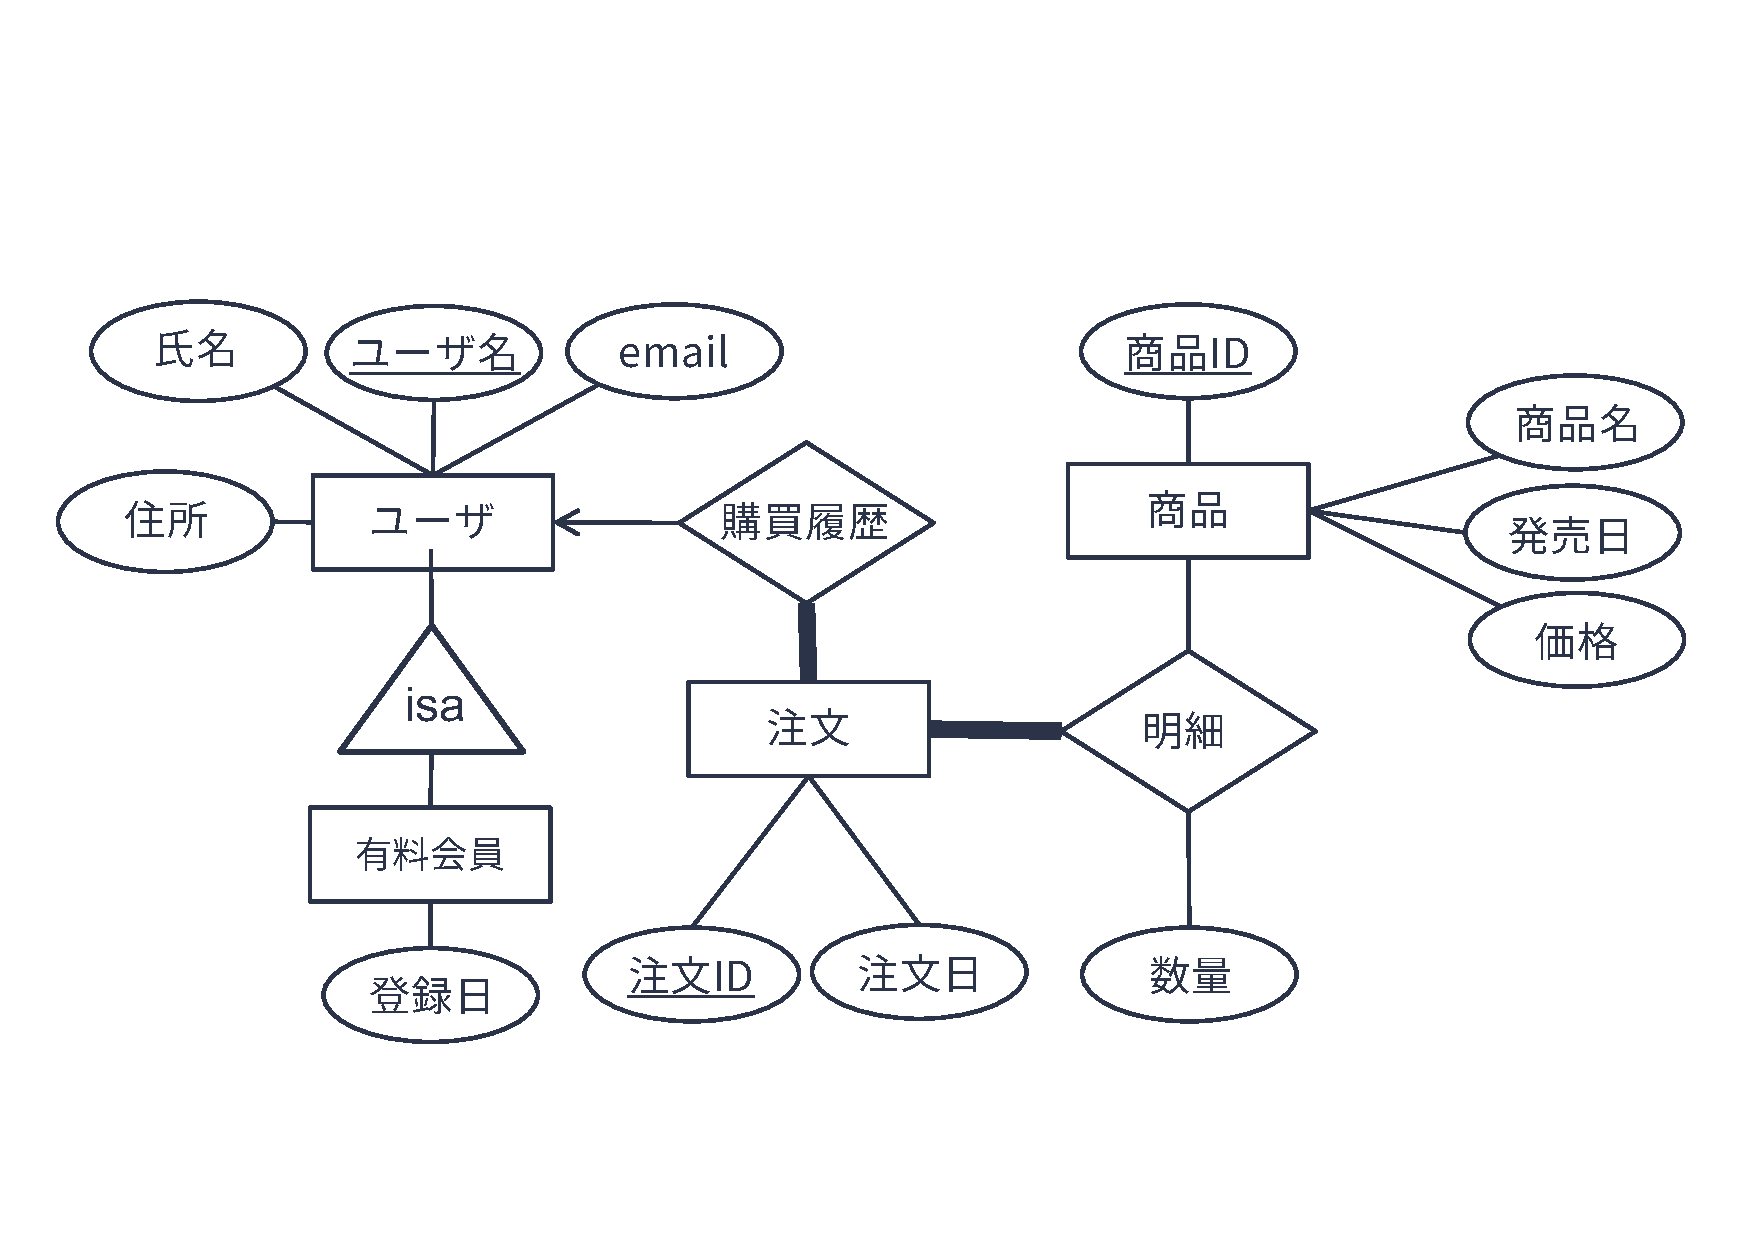
\includegraphics[width=1.0\textwidth]{figure/er-model/erd-to-schema.pdf}
    \caption{購買履歴を管理するシステムの実体関連図}
    \label{fig:erd-to-schema}
\endfigure
